\documentclass[]{final_report}
\usepackage{graphicx}
\graphicspath{ {./images/}{../../media/images} }
\usepackage{hyperref}
\usepackage{amssymb}
\usepackage{amsmath}
\usepackage{dirtytalk}
\usepackage{calligra}
\usepackage{subcaption}
\usepackage{float}


\usepackage{fancyvrb}
\newcommand{\VerbBar}{|}
\newcommand{\VERB}{\Verb[commandchars=\\\{\}]}
\DefineVerbatimEnvironment{Highlighting}{Verbatim}{commandchars=\\\{\}}
% Add ',fontsize=\small' for more characters per line
\newenvironment{Shaded}{}{}
\newcommand{\AlertTok}[1]{\textcolor[rgb]{1.00,0.00,0.00}{\textbf{#1}}}
\newcommand{\AnnotationTok}[1]{\textcolor[rgb]{0.38,0.63,0.69}{\textbf{\textit{#1}}}}
\newcommand{\AttributeTok}[1]{\textcolor[rgb]{0.49,0.56,0.16}{#1}}
\newcommand{\BaseNTok}[1]{\textcolor[rgb]{0.25,0.63,0.44}{#1}}
\newcommand{\BuiltInTok}[1]{#1}
\newcommand{\CharTok}[1]{\textcolor[rgb]{0.25,0.44,0.63}{#1}}
\newcommand{\CommentTok}[1]{\textcolor[rgb]{0.38,0.63,0.69}{\textit{#1}}}
\newcommand{\CommentVarTok}[1]{\textcolor[rgb]{0.38,0.63,0.69}{\textbf{\textit{#1}}}}
\newcommand{\ConstantTok}[1]{\textcolor[rgb]{0.53,0.00,0.00}{#1}}
\newcommand{\ControlFlowTok}[1]{\textcolor[rgb]{0.00,0.44,0.13}{\textbf{#1}}}
\newcommand{\DataTypeTok}[1]{\textcolor[rgb]{0.56,0.13,0.00}{#1}}
\newcommand{\DecValTok}[1]{\textcolor[rgb]{0.25,0.63,0.44}{#1}}
\newcommand{\DocumentationTok}[1]{\textcolor[rgb]{0.73,0.13,0.13}{\textit{#1}}}
\newcommand{\ErrorTok}[1]{\textcolor[rgb]{1.00,0.00,0.00}{\textbf{#1}}}
\newcommand{\ExtensionTok}[1]{#1}
\newcommand{\FloatTok}[1]{\textcolor[rgb]{0.25,0.63,0.44}{#1}}
\newcommand{\FunctionTok}[1]{\textcolor[rgb]{0.02,0.16,0.49}{#1}}
\newcommand{\ImportTok}[1]{#1}
\newcommand{\InformationTok}[1]{\textcolor[rgb]{0.38,0.63,0.69}{\textbf{\textit{#1}}}}
\newcommand{\KeywordTok}[1]{\textcolor[rgb]{0.00,0.44,0.13}{\textbf{#1}}}
\newcommand{\NormalTok}[1]{#1}
\newcommand{\OperatorTok}[1]{\textcolor[rgb]{0.40,0.40,0.40}{#1}}
\newcommand{\OtherTok}[1]{\textcolor[rgb]{0.00,0.44,0.13}{#1}}
\newcommand{\PreprocessorTok}[1]{\textcolor[rgb]{0.74,0.48,0.00}{#1}}
\newcommand{\RegionMarkerTok}[1]{#1}
\newcommand{\SpecialCharTok}[1]{\textcolor[rgb]{0.25,0.44,0.63}{#1}}
\newcommand{\SpecialStringTok}[1]{\textcolor[rgb]{0.73,0.40,0.53}{#1}}
\newcommand{\StringTok}[1]{\textcolor[rgb]{0.25,0.44,0.63}{#1}}
\newcommand{\VariableTok}[1]{\textcolor[rgb]{0.10,0.09,0.49}{#1}}
\newcommand{\VerbatimStringTok}[1]{\textcolor[rgb]{0.25,0.44,0.63}{#1}}
\newcommand{\WarningTok}[1]{\textcolor[rgb]{0.38,0.63,0.69}{\textbf{\textit{#1}}}}
\usepackage{longtable,booktabs}

\setlength{\emergencystretch}{3em} % prevent overfull lines
\providecommand{\tightlist}{%
  \setlength{\itemsep}{0pt}\setlength{\parskip}{0pt}}



%%%%%%%%%%%%%%%%%%%%%%
%%% Input project details
\def\studentname{Cougar Tasker}
\def\reportyear{2023-24}
\def\projecttitle{Effective Exploration in Markov Decision Processes}
\def\supervisorname{Dr. Anand Subramoney}
\def\degree{MSci (Hons) in Computer Science (Artificial Intelligence)}
\def\fullOrHalfUnit{Full Unit} % indicate if you are doing the project as a Full Unit or Half Unit
\def\finalOrInterim{Final Report} % indicate if this document is your Final Report or Interim Report

\begin{document}

\maketitle

%%%%%%%%%%%%%%%%%%%%%%
%%% Declaration

\chapter*{Declaration}

This report has been prepared on the basis of my own work. Where other published and unpublished source materials have been used, these have been acknowledged.

\vskip3em

Word Count: 14,055 (16,043 including appendix)

\vskip3em

Student Name: \studentname

\vskip3em

Date of Submission: 05/04/2024

\vskip3em

Signature: {\calligra \LARGE \studentname}

\newpage
\vspace*{\fill}
\begin{center}
  \begin{minipage}{0.7\textwidth}
    \raggedright % Left align the text
    Dedicated to my partner, friends and family:\\
    Thank you for your continued support and encouragement.
  \end{minipage}
\end{center}


\vspace*{\fill}
\newpage

%%%%%%%%%%%%%%%%%%%%%%
%%% Table of Contents
\tableofcontents\pdfbookmark[0]{Table of Contents}{toc}\newpage

%%%%%%%%%%%%%%%%%%%%%%
%%% Your Abstract here

\begin{abstract}
  
  Reinforcement Learning (RL) is a machine-learning paradigm, like supervised and unsupervised learning. In Reinforcement Learning, the agent makes decisions and receives judgment in this fashion, which is similar to supervised learning. However, in reinforcement learning, this judgment is provided after the agent decides on the consequences of their actions. There is also no distinction between training and testing. Instead, the agent continuously learns from their successes and failures. RL is also unlike unsupervised learning; its agents operate within the system rather than observing patterns. Furthermore, unlike unsupervised learning, reinforcement learning has an objective: to learn to achieve more rewards. Reinforcement Learning is also built upon a robust mathematical foundation that aids in the research and development of the field and allows us to make some strong guarantees. Furthermore, RL has a broad reach, uniting many important and diverse areas of study such as Economics, Optimisation, Game Theory, Robotics, and Cognitive Science. 

  These unique differences in reinforcement learning, especially its ability to learn through interactions,  make this field applicable to many real-world problems. For example, RL is applied to problems within Transportation, Robotics, Healthcare, Finance, and more~\cite{RLapplications}. However, these differences also introduce new challenges, such as the delayed reward, which complicates updating the agent. Furthermore, the information the agent learns depends upon the agent's actions; therefore, to learn efficiently, the agent would benefit from knowing the environment. In other words, to gain knowledge efficiently, the agent must already have the knowledge. When the rewards are sparse, this learning problem is analogous to an explorer searching for treasure; the explorer can be far more efficient if they have a rough treasure map. 
    
  It follows that the primary goal of this project is to understand and implement reinforcement learning. Furthermore, the secondary goal is to discern how these agents explore and the challenges faced in doing this efficiently. Of these challenges, this report focuses on how hyper-parameter tuning impacts exploration and the problems and opportunities it presents. This report also compares the performance characteristics of three exploration strategies of varying complexity and sophistication. From this, it is shown that with substantial tuning, even the most straightforward strategy can perform at a similar level as the state-of-the-art. However, this constitutes a form of overfitting, and the real benefit of these advanced algorithms is their generalisation ability. 
  
\end{abstract}

%%%%%%%%%%%%%%%%%%%%%%
%%% Introduction 

\chapter{Introduction}

This report documents a study into reinforcement learning and exploration of markov decision processes. This project can broadly be broken into three components: research, implementation and analysis. The report documents the research component in three main parts. The literature review section~(\ref{sect:literature-review}) covers all of the main literature used throughout the research. The professional issues chapter~(\ref{chap:professional-issues}) discusses social and ethical issues in reinforcement learning and the related research. The Fundamental Concepts chapter~(\ref{chap:fundamental-concepts}) explains reinforcement learning concepts with ties to the relevant literature. Details of the implementation are documented in the software engineering chapter~(\ref{chap:software-engineering}). There are two parts to the analysis component, firstly the exploration strategy effectiveness chapter~(\ref{chap:exploration-strategy-effectiveness}) documents an analysis of the results and the final chapter~(\ref{chap:project-analysis}) analyses the project as a whole.

\section{Aims and Objectives}

This section extends on the projects primary objective of understanding and implementing reinforcement learning from the abstract and covers the main deliverables from the project requirements. The main aim of this project is to implement agents that can learn to operate in a Markov decision process. Each agent must be based on an existing algorithm in the reinforcement learning literature. These agents must be adaptable, they must not use any environment-specific techniques or knowledge. In other words, these agents must generalise well, therefore they must be tested in different environments.

The program must make the learning system accessible to the user, The user must be able to interpret what is happening and be able to control factors of the system. This must be achieved with an animated user interface and configuration file. Furthermore, the application must collate together results from the simulations and present this to the user in a form that facilitates analysis. It must be possible to export these results for use in the report. 

Finally with results drawn from this application an analysis and comparison of different exploration strategies should be performed. This analysis should cover the details of how efficiently each agent has explored and provide the reader with an understanding of any uncertainty in the results. This report should document all parts of the process, from background research to conclusions. This report must include an explanation of the reinforcement learning background as well as describing the software engineering processes involved.

\newpage
\section{Motivations}

My inspiration for studying for this degree, specialising in artificial intelligence, comes in large part from my belief that AI is becoming increasingly pivotal in shaping the future of technology and industry. For this purpose, this project presents an invaluable opportunity for my personal and professional growth. It is a fantastic platform to improve my comprehension of reinforcement learning while offering hands-on experience. 

Last year, I completed my year-long internship at Zing Dev (Zing), a digital communications company that is progressively incorporating AI systems for its customers. This experience has demonstrated to me the value of understanding the internals of these AI systems. It is clear that AI is a clear focus for most companies, Ransbotham et al. said: 
\begin{quote}
  Almost 85\% believe AI will allow their companies to obtain or sustain a competitive advantage~\cite{ransbotham2017reshaping}
\end{quote}

Through this project, I aim to improve my understanding of autonomous agents' benefits, biases, and limitations. This knowledge will be desirable for many companies like Zing working with artificial agents.


\section{Literature Review}\label{sect:literature-review}

This section reviews the relevant literature on Reinforcement Learning as well as some of the broader fields of Artificial Intelligence (AI) and Machine Learning (ML). The literature selection focuses on the foundations of RL and its potential ethical and societal implications.

Implementing RL algorithms is central to this project. Several studies provide a foundation in core concepts such as the Bellman equations~\cite{bellman1957}, Markov Decision Processes (MDPs)~\cite{meyn2012markov,sutton2018reinforcement}, Q-learning~\cite{watkins1992q}, and double Q-learning~\cite{doubleQLearning}. Notably, the comprehensive text \say{Reinforcement Learning: An Introduction} by Sutton and Barto~\cite{sutton2018reinforcement} offers a wide-ranging exploration of RL, touching upon most topics covered in this report. In 1989 Watkins introduced Q-learning, in this original paper the reward was provided in a secondary function separate from the environment~\cite{watkins1992q}. While this two-function approach is technically identical to the combined notation of Sutton it is less concise in the Bellman equations and can obscure the relationship between environment and rewards. For these reasons, this report will use Sutton's single probability distribution notation.

Reinforcement Learning has several challenges inherent to the field, including the exploration-exploitation dilemma. The \say{RBED} paper~\cite{rewardEpsilonDecay} introduces a new reward-based approach to managing this dilemma, however, the paper only demonstrates improved reward at the end of the episode when compared with exponential decay. It seems substantially worse with short episodes and the paper does not make any comparison with a linear decay to which it seems the most similar. Furthermore, this approach introduces more tunable hyperparameters than the traditional approaches.

Several other studies address different technical hurdles, including convergence~\cite{watkins1992q, QlearningConvergance}, and hyperparameter tuning~\cite{deepRLChallanges, searchStrategies}. Others delve into the specifics of deep reinforcement learning, exploring its definition~\cite{deepRLOverview} alongside the challenges associated with its development, such as instability~\cite{deepOnVsOffPolicy,sutton2018reinforcement} and the difficulty and expense of tuning~\cite{deepRLChallanges, DeepRLCost}. Additionally, some studies bridge the gap between RL and psychology, investigating its connection to the theory of operant conditioning~\cite{shteingart2014reinforcement,staddon2003operant}.

A core aspect of this project is effective exploration. Numerous studies grapple with the complex issue of accurately measuring performance and address methods to account for or avoid hyperparameter tuning difficulties~\cite{assessingDeepRL, evaluatingRL, parameterFreeExploration}. Further studies explore strategies to optimise an agent's learning process by setting appropriate learning rates and initial values~\cite{even2003learning, deathTransfer,decayingLearningRates}. The \say{aRtificiaL death} paper~\cite{deathTransfer} covers the interesting idea of using the experience of previous or \say{dead} agents to provide the initial values of new agents. The results provided in this paper are interesting however, it is not clear what the impact of the unusual \say{Novelty Seeking Agent} is. It would have been informative to also see the impact of using a more standard agent such as $\varepsilon$-greedy.

The choice of exploration strategy significantly impacts the efficiency with which a Q-learning agent explores its environment. The book by Sutton and Barto~\cite{sutton2018reinforcement} covers many standard exploration options. Notably, the paper \say{Model-Free Active Exploration in Reinforcement Learning}~\cite{modelFree} introduces a cutting-edge exploration strategy based on the best policy identification problem~\cite{bestPolicyIdentifaction}. Another study establishes the characteristic time measure~\cite{characteristicTime} that underpins this strategy. However, a different study demonstrates that this measure is non-convex~\cite{characteristicTimeNonConvex}, making it challenging to solve and directly incorporate into an exploration strategy. While the MF-BPI paper~\cite{modelFree} is built upon this prior work of the BPI problem it seems omit some details at how it has reached its algorithm, The theoretical work is based upon knowing certain quantities that would be unknown to the algorithm. Furthermore, while the paper demonstrates that it is competitive to other strategies, it is only done in their own and new \say{Forked Riverswim} environment. It would have been compelling to show a variety of standard environments.

Software engineering principles are essential to this project, providing a structured approach to developing robust software. Several papers discuss the fundamental principles of software engineering and their practical application~\cite{softwareEngineringPrinciples,van2008software}. Unit testing, a cornerstone of software engineering, is evaluated in a survey that highlights its strengths and limitations~\cite{unitTestingSurvey}. The application utilises a Model-View-Controller (MVC) architecture variant, and several papers explore similar architectures~\cite{webMVC, mvvm, gamesMVC}. Finally, a study examines the technical considerations involved in creating machine learning applications using Python~\cite{pythonMachineLearning}. Two additional papers delve into aspects of modern software development: development containers~\cite{developmentContainers} and Python best practices such as inline documentation~\cite{pythonAutoDoc}.

The following chapter~(\ref{chap:professional-issues}) will analyse the social and ethical implications of RL and the broader field of machine learning. Several studies provide a detailed examination of the Amazon \say{Rekognition} case study~\cite{facialRecognitionBias, legislatingRekognition, legislatingOG, rekognitionOverview}. A number of papers emphasise the potential social harms arising from biased and unbiased ML models~\cite{AISocialImpactAndAccountability,facialRecognitionBias, anprAccountability}. Several studies explore how ML programs inherit biases from their training data~\cite{LLMSocialEthicalRisks, AISocialImpactAndAccountability, facialRecognitionBias}. Two studies explore the military applications of RL, such as its use in unmanned aerial vehicles~\cite{rlMilitaryReviewChina, DRLDrones}. Finally, a select few papers discuss the potential benefits RL offers to society and propose principles that could aid in mitigating the risks associated with this technology~\cite{AIRisksAndPrinciples,deepRLsocietalImpact, ransbotham2017reshaping}.

\chapter{Professional Issues in Machine Learning}
\label{chap:professional-issues}

Machine learning programs and techniques, as explored in this project, possess immense potential for social benefit when managed judiciously, but they also risk significant social and ethical consequences~\cite{AISocialImpactAndAccountability}. One concern is the ability of ML systems to reinforce and perpetuate societal biases in their decisions~\cite{AISocialImpactAndAccountability}. One prominent example of this dichotomy of potential was \say{Rekognition}, Amazon's facial recognition tool (FRT)~\cite{legislatingOG}. Rekognition is a cloud-based deep-learning application which can identify people, activities, objects, and more~\cite{rekognitionOverview}. This powerful tool can bring societal benefit one example is an application that notifies professionals who are in high-risk sectors such as healthcare or construction~\cite{rekognitionOverview}. Rekognition can make this possible by detecting Personal Protective Equipment. 

Recent developments in AI have spurred many companies such as IBM, Microsoft, and Amazon to release FRTs, making identification more convenient than ever~\cite{facialRecognitionEthicsSurvay}. While there have been many commercial applications, the most notable example from a moral, ethical and social standpoint was the use of Rekognition by US law enforcement agencies. From 2018-2020 the FBI trailed Rekognition to assist in searching video footage collected during investigations~\cite{facialRecognitionBias}. Other agencies such as the DEA use FRTs to help identify criminals captured on surveillance cameras~\cite{facialRecognitionBias}. 

So why is this significant? Unfortunately, Rekognition's social impact has not been wholly positive; it has tended to falsely identify women and people of colour as criminals to a disproportionate degree~\cite{legislatingRekognition}. Moreover, it falsely identified twenty-eight NFL players as
criminals, of which thirteen were persons of colour~\cite{facialRecognitionBias}. While human oversight may be used, it is not enough. These errors have already led to serious harm, and the significant bias to race and sex is discriminatory and unacceptable.

While the intentions of operators and machine learning professionals may be for social good it is evident that without careful consideration machine learning systems may not be aligned with our goals~\cite{AIAllignemnt}. In the context of FRT, it is clear there had been several compounding failures. Firstly it can be easy to believe that your ML system is unbiased and avoid responsibility when your algorithms are generalised and independent of any particular protected characteristic. However, vendors such as Amazon provide these ML systems pre-trained as a service. For ML models their training data can be the largest determinant of their functionality. 

\begin{quote}
  Bias in, Bias out~\cite{facialRecognitionBias}
\end{quote}

\begin{quote}
  For Microsoft, almost ninety-four percent of
  the faces misgendered were individuals who were considered darker individuals~\cite{facialRecognitionBias}
\end{quote}

Biases in training datasets propagate to the decisions made by the model it is trained on. These biases in the error rate are believed to be a consequence of an over-representation of some social identities in the training data~\cite{LLMSocialEthicalRisks}. Gathering more data has been long considered the goal in ML for creating better models, particularly large language models which have been directly trained on large corpora of text from the internet~\cite{LLMSocialEthicalRisks}. However, it's my belief that fair and equal representation of all protected characteristics should be a top priority even at the expense of discarding data.

\newpage
While reducing biases in training is incredibly important and achievable, with datasets at scale it may be impractical or impossible to truly remove all bias. We must acknowledge and account for the shortcomings of ML systems. This is especially important where AI systems make decisions that impact people. The FBI's system involved human oversight and intervention and yet people of colour were still disproportionately harmed. In fact, in another example, even a truly unbiased technology, automatic number plate recognition (ANPR) has been found to cause a disparate impact on people of colour~\cite{anprAccountability}. The implicit biases of the operators resulted in this technology being used in higher frequency in Black and Latinx communities~\cite{anprAccountability,facialRecognitionBias}.

While the human factor of implicit biases makes them harder to tackle systematically, I believe several steps can be taken in machine learning to reduce  the aforementioned issues:
\begin{itemize}
  \item Unbiased systems as default, where using protected characteristic data is not necessary or avoidable, then this information should be removed where possible~\cite{AIRisksAndPrinciples}. This may be possible to achieve with redaction or masking in some contexts.
  \item Active training management, ensuring equality in training datasets that include people's protected characteristics. This may be achieved by sampling and further models to categorise data~\cite{AIRisksAndPrinciples}.
  \item Algorithmic bias awareness, trained ML systems must have their bias quantified before their use. Stakeholders must be made aware of the system's limitations before it is approved~\cite{AIRisksAndPrinciples}.
  \item Implicit bias awareness, operators of ML systems should receive continuous training and feedback to ensure that they are aware of their own implicit biases and the impact of their decisions~\cite{facialRecognitionBias}.
  \item Transparency and accountability: decision-makers at every stage of ML systems should be transparent about the decisions that they have made and accountable to the people that these decisions affect~\cite{AIRisksAndPrinciples}.
\end{itemize}
AI must be regulated in a fashion where we no longer perpetuate existing or create new social harms while not discouraging the potential societal benefits that it may bring~\cite{AIRisksAndPrinciples}. 


This case study is one of many that may highlight similar or different challenges and benefits that AI may bring. Unlike the case study, the application in this project is exploratory and operates in simulated environments. In this sense, I believe it is insulated from bias and causes this type of social harm. However, this is just one facet of how these systems incorporate with society. Like machine learning as a whole RL, specifically deep reinforcement learning (DRL), increasing use to solve practical problems~\cite{deepRLsocietalImpact}. One place DRL is being applied is in militaries across the world~\cite{rlMilitaryReviewChina, DRLDrones}. Of these military applications, their use in UAVs has seen impressive success. In DARPA's AlphaDogfght competition, an autonomous DRL agent beat a human F-16 pilot 5:0 and won the championship~\cite{rlMilitaryReviewChina}. These UAVs have grown in their autonomous capabilities~\cite{DRLDrones} and it's clear that in conflicts these agents may operate weapons systems. When a reinforcement learning agent's action space includes taking a human life, is this morally and ethically right?

These systems may have been trained in a simulation of military operations and rewarded for their actions that achieved military goals~\cite{rlMilitaryReviewChina}. These experiences will shape the agent's interpretation of value. But, these experiences are unlike ours as humans. As humans, we have a vast variety of experiences, including companionship and kindness. In this respect, the value a human and DRL combatant will assign to killing their opponents may differ vastly. I believe there may be situations where an AI may pick actions that may lead to a devastating loss of life for only a miniscule increase in the chance of success. 

\chapter{Fundamental Concepts}
\label{chap:fundamental-concepts}
\section{Markov Decision Processes}

Markov Decision Processes (MDP) provide a mathematical formalisation of decision-making problems. Markov Decision Processes provide the foundation for reinforcement learning (RL). This is because MDPs distil the fundamental parts of decision-making, allowing RL techniques built upon MDPs to generalise to learning in the real world and across different domains such as finance and robotics~\cite{RLapplications}. 

As a formal mathematical framework, MDPs allow us to derive and prove statements about our RL methods built upon them. An important example of this is that we can prove that Q-learning (an RL technique explained in chapter~\ref{sect:q-learning}) will converge to the true Q-values as long as each Action-State pair is visited infinitely often~\cite{watkins1992q}. Furthermore, MDPs allow us to reason about problems with uncertainty, allowing RL agents to account for randomness in their environment. 

The standardisation of decision-making problems as MDPs allows for a uniform definition of optimality with the value functions. MDPs give a basis for assessing the performance of RL algorithms, facilitating like-for-like comparisons for different RL approaches. 


\subsection{Markov Property}

The Markov property is that the future state of a Markov system only depends on the current state of the system. In other words, if we have a system that follows the Markov property, then the history preceding the system's current configuration will not influence the following state.

To put the Markov property formally, $S_t$ represents the state at some time as $t$. $S_t$ represents the outcome of some random variable. Then the Markov property would hold if and only if:


\begin{equation}
  \Pr(S_{c+1}\ |\ S_{c},S_{c-1},\dots,S_0) = \Pr(S_{c+1}\ |\ S_{c})
  \label{eqn:markov-property}
\end{equation}

This definition demonstrates how the Markov property can hold in non-deterministic, stochastic processes. It also shows that predictions that are only based on the current state are just as good as those that record the history in a Markov process. The sequence of events in this definition, $S_t$, is called a Markov Chain~\cite{meyn2012markov}.

\newpage
\subsection{Extending Markov Chains}

Markov Decision Processes extend Markov Chains in two important ways. Firstly, MDPs introduce decision-making through actions. Each state in an MDP has a set of actions available to it. In each state, an action is required to transition to the next state; this action with the current state can affect what the following state will be. Secondly, MDPs introduce a reward value. The reward is determined from the current state and action; it is produced simultaneously with the following state.

A formal definition of a Markov Decision Process is a tuple $(\mathcal{S},\mathcal{A}_s,p)$ where:
\begin{itemize}
  \item $\mathcal{S}$ defines the set of all states
  \item $\mathcal{A}_s$ defines the set of available actions in state $s$
  \item $p$ defines the relationship between states, actions and rewards: \\
        $p(s',r\ |\ s,a) \doteq \Pr(S_{t+1} = s', R_{t+1} = r | S_t = s, A_t = a)~\cite{sutton2018reinforcement}$
        \begin{itemize}
          \item $s, s' \in \mathcal{S}$, $a \in \mathcal{A}_s$ and $r \in \mathbb{R}$
          \item $p: \mathcal{S} \times \mathbb{R} \times \mathcal{S} \times \mathcal{A} \rightarrow [0,1]$
        \end{itemize}
\end{itemize}

The function $p$ is an integral part of this definition; it fully describes how the system will evolve. We call this function the dynamics of the MDP. What this definition does not describe is how actions are chosen. This decision-making is done by an entity called an agent. For our purposes, the agent will have complete visibility as to the current state of the MDP. However, like most real-world situations, our agent will not have any a priori knowledge of the dynamics. 

\begin{figure}[H]
  \centering
  
  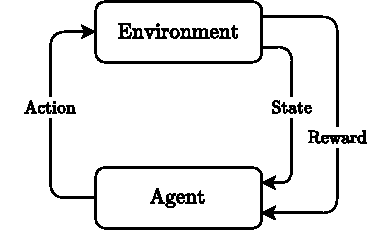
\includegraphics[width=8cm]{agent-enviroment-2}
  
  \caption{\label{fig:agent-enviroment} The agent-environment interface}
\end{figure}

The agent comprises the entire decision-making entity in an MDP; anything unknown or not wholly under the agent's control is called the agent's environment. In the context of reinforcement learning, the environment is essentially the dynamics of the MDP. Figure~\ref{fig:agent-enviroment} demonstrates how the agent and environments affect each other in an MDP. 

\label{policy-informal-definition}
For learning agents, we wish to improve the agent's behaviour over time. For this purpose, we introduce a policy $\pi$. This policy defines the action chosen by an agent under a particular state. The policy can be represented with a lookup table like in Q-learning~(\ref{sect:q-learning}) or a more complex process such as deep Q-learning. A policy like this is not hard-coded, allowing the agent to update the policy based on the information the agent learns from the environment. 


\section{Policy and Value Functions}

After each action, a reward is received. It follows that the goal of an agent should be to choose the actions to maximise these reward signals received. Following the Markov principle and the definition of an MDP, this reward only depends on the current state and the action chosen. Consequently, being in some states and performing some actions are more valuable to the agent than other states and actions. We can define value functions: 
\begin{itemize}
  \item $v(s)$ function determines the value of being in a given state
  \item $q(s, a)$ function determines the value of being in a given state and performing a specific action
\end{itemize}



\begin{figure}[H]
  \centering
  
  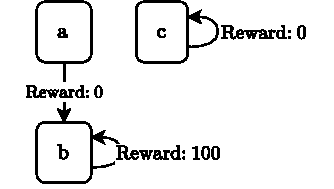
\includegraphics[width=8cm]{reward-example-2}
  
  \caption{\label{fig:reward-example} An example of transitive value of states $v(b) > v(a) > v(c)$}
\end{figure}

Intuitively, the value of being in a state is more than only its immediate reward that might be found from performing actions in that state. It is also related to the potential future reward that might be achieved in the reachable subsequent states. This can be demonstrated with two states $a$, and $b$, where there is a large reward at $b$ and the only way to reach $b$ is through $a$. It is clear that despite the identical immediate rewards, the state $a$ is more valuable than $c$ due to future potential at $b$ available at $a$. However, $a$ can be considered less valuable than $b$ because more steps are always required to achieve the reward from $a$ than at $b$. To account for this preference for more immediate rewards, the value function should also discount future value with a parameter $\gamma$. 

These value functions go hand in hand with an agent's policy; a good policy maximises being in valuable states and performing valuable actions. On the other side of the coin, the value is determined by the subsequent states and rewards, which are in part determined by the actions the policy selects. Basing the policy on the value function gives the value function's definition impact over that agent's decision-making, in particular, the\label{discount-rate-introduction} discount rate ($\gamma$). With high discount rates $\gamma \approx 1$, the agent can be far-sighted and ignore short-term high-reward actions available to it and take longer to learn. With low discount rates $\gamma \approx 0$, the agent can be short-sighted, ignoring the potential long-term benefits of specific actions.

While the policy is informally described at the end of chapter~\ref{policy-informal-definition}, a formal definition of a policy ($\pi$) is the probability distribution of an agent picking a given action in a given state:

\begin{equation}
  \pi(a \ |\ s) \doteq \Pr(A_t = a | S_t = s)
  \label{eqn:policy-def}
\end{equation}



Where $s \in \mathcal{S}$ and $a \in \mathcal{A}_s$. This definition shows how the policy can be stochastic. A stochastic policy can be beneficial in many ways, such as breaking ties where multiple actions are equally good and choosing between when to explore more or seek rewards. 

\subsection{Optimal Policy/Value Function via the Bellman Equation}

With a known policy and dynamics, the future state can be wholly determined, allowing for a complete mathematical definition of the value functions under a given policy that describes our above intuitions. for the state-value function ($v$) and action-value function ($q$) under a policy $\pi$ we have the formulas:


\begin{align}
  q_\pi(s,a) & \doteq \sum_{s',r}p(s',r\ |\ s, a)[r + \gamma v_\pi(s')]\label{eqn:q-def} \\
  v_\pi(s)   & \doteq \sum_a \pi(a\ |\ s) q_\pi(s,a) \label{eqn:v-def}
\end{align}

These value functions are defined recursively in terms of each other; these definitions can be unrolled to only be in terms of themselves. The unrolled form of the state-value function is known as the Bellman equation. These equations are named Richard Bellman, who, in the process of developing the field of dynamic programming, created them~\cite{bellman1957}.   

These functions demonstrate the intertwined relationships between the policy chosen and the value of that state if there is a particularly valuable action $a^\star$ such that $q_\pi(s,a^\star)$ is far better than for all other actions. A policy $\pi(a^\star\ |\ s) = 0$ would hamper the potential value of $s$. Therefore, the value function can be used to compare how well different policies perform. If for policy $\pi_a$ there does not exist another policy $\pi_b$ such that $\pi_b$ has a better value $v_{\pi_b}(s) > v_{\pi_a}(s)$ for all states $s \in \mathcal{S}$ then we can consider this policy $\pi_a$ an optimal policy. There may be many optimal policies; however, we often do not need to distinguish them, so we often denote any optimal policy with $\pi_\star$. This is because all optimal policies share the same state-value, and by definition action-value, function, we denote this $ v_\star$ and $q_\star$. The optimal value function $v_\star$ is known as the Bellman optimality equation. These optimal equations can be written formally as:


\begin{align}
  q_\star(s,a) & \doteq \max_\pi q_\pi(s,a)\label{eqn:q-optimal-def} \\
  v_\star(s)   & \doteq \max_\pi v_\pi(s) \label{eqn:v-optimal-def}
\end{align}




\subsection{Finding Optimal Policies by Iteration}\label{iteration-approaches}

Although optimal policies exist, finding them is another matter. The policy search space is potentially infinite, so an intelligent method is required. An optimal policy can be extracted from an optimal value function and the dynamics of the MDP; the optimal policy would only select actions that result in the highest value. Finding the optimal value function with the optimal policy is straightforward, but this is a catch-22. The optimal value function must be self-consistent with the Bellman equations. One approach to solving these equations is iteration, for each step moving slightly closer to the optimal solution from an initial guess. 

\newpage
\subsubsection{Policy Iteration}

In policy iteration, we improve a policy over time until it is optimal. Updating a policy like this is only possible because of the policy improvement theorem. This theorem considers if we have a policy $\pi_{\text{old}}$. We are at some state $s$, $\pi_{\text{old}}$ will pick the action $a$ under this state $\pi_{\text{old}}(a\ |\ s) = 1$ what happens if we consider some other action $a'$ but then continue to follow the original policy. Because we continue to follow the original policy, we can use the existing value function $v_{\pi_{\text{old}}}(S_{t+1})$ for the subsequent states. We call this slightly adjusted policy $\pi_{\text{new}}$. By applying the Bellman equations and the existing value function we can recalculate the value at $s$ of $\pi_{\text{new}}$ if this new value is better than the original policy then we know that $\pi_{\text{new}}$ must be as good if not better for all states $s \in \mathcal{S}$ than $\pi_{\text{old}}$ thus $\pi_{\text{new}}$ would be a better policy. 


\begin{equation}
  \sum_a \pi_{\text{new}}(a\ |\ s) q_{\pi_{\text{old}}}(s,a) \ge v_{\pi_{\text{old}}}(s) \Rightarrow  \pi_{\text{new}} \ge \pi_{\text{old}}
  \label{eqn:policy-improvement-theorem}
\end{equation}

For some policy $\pi$ you can apply this policy improvement theorem for every state and action in the MDP. This approach of comparing all actions over all states is called policy improvement. This policy improvement step can be applied iteratively until the policy stops improving. If the policy does not improve over this policy improvement step, then all of the actions are optimal, and this policy is optimal

Although this policy improvement sounds computationally expensive, each state can be considered simultaneously and with a shared base policy; in each iteration, the state-value function is the same; caching this removes redundant calculations. Calculating the value function is improved by using an iterative approach and utilising the previous value function as a launching point.  


\subsubsection{Value Iteration}

Policy iteration is a practical approach, for a finite MDP is guaranteed to finish in finite time. In practice, policy improvement does better and only takes a few iterations. However, in each iteration, multiple full sweeps of the state space are required. The idea of Value Iteration is to improve the policy within the Value Iteration step. This Value Iteration approach only requires one iteration. 

The Bellman equation~(\ref{eqn:v-def}) can be used as an update rule to compute the value function iteratively. A table of values is maintained for each state, initialised randomly. The value of each state can be updated based on the immediate reward and the current estimates of the subsequent states; this is guaranteed to reduce the error at that state because the $\gamma$ discount rate discounts the error at the subsequent state. This process is called bootstrapping; the smaller $\gamma$, the quicker the error rate will decrease, and the faster the process will converge. When the inconsistency at each state is suitable, the process will stop. 

This standard approach uses the traditional value Bellman equation~(\ref{eqn:v-def}) to find the value for a given policy. In value iteration, there is an implicit policy that exclusively picks the action that has the maximum value. This policy is optimal for the optimal value function; when the Value Iteration converges, it must be optimal because of these conditions. This augmented update rule can be defined as:

\begin{align}
  q_{\text{max}}(s,a)          & \doteq \sum_{s',r}p(s',r\ |\ s, a)[r + \gamma v_{\text{max}}(s')] \tag{from~\ref{eqn:q-def}} \\
  v_{\text{max}}(s)            & \leftarrow  \max_a q_{\text{max}}(s,a) \label{eqn:v-update}                                  \\
  \therefore v_{\text{max}}(s) & \leftarrow  \max_a \sum_{s',r}p(s',r\ |\ s, a)[r + \gamma v_{\text{max}}(s')]
\end{align}


As this new update rule involves no explicit policy, a final step is required in Value Iteration to extract an explicit policy. In this step, the action that leads to the best value for each step, according to the $q_\star$ function.$q_\star$, can be derived from the $v_\star$ with the dynamics $p$ function.


\section{Learning as Incrementally Optimising a Policy in a MDP}

Learning is the process of acquiring new information and skills. There are many different ways organisms can learn. In psychology, one of the methods is operant conditioning. In Operant Conditioning, the learner receives feedback from the environment as either a reward or punishment for completing different actions~\cite{staddon2003operant}. In an experiment, this could be some food for opening a door, and this feedback influences the learner's future actions. This mechanism has equivalences to reinforcement learning. For this reason, RL is considered the dominant theoretical framework for operant learning~\cite{shteingart2014reinforcement}. 

To demonstrate learning as policy optimisation, consider an agent that is introduced to a new Markov environment. This agent has no prior knowledge; therefore, its initial policy is independent of the environment's features. Eventually, the agent will pick some action in a state and receive some reward from the environment. This information can be used to update the policy and prioritise one successful action. Since the environment obeys the Markov property, repeating this successful action will continue to reward. If the agent continues to optimise its policy as it finds rewards, then it can improve its average reward. Through incrementally optimising its policy, this agent has learnt which actions are more successful and improved its behaviour.

\section{Q-Learning}\label{sect:q-learning}


Q-learning is like value and policy iteration; all search for an optimal value function. However, Q-learning operates under extra constraints. The value and policy iteration extensively use the MDP's dynamics ($p$). In most real-world problems, the dynamics are unknown or too complex to be represented accurately. Iteration approaches can be adapted using samples to work without $p$. Samples are captured from the environment when the agent performs actions, which can be chosen randomly or by following another policy. Monti-Carlo is another technique that uses samples to emulate the value functions more directly, but these approaches are inherently offline. While offline methods have many advantages, their shortcomings, such as the inability to adapt to changing environments, make them unsuitable for many applications. 

\subsection{Temporal difference}

Temporal difference (TD) algorithms are another class of RL algorithms. TD is an online process that improves the policy as new data becomes available. The goal of TD is to minimise the $\delta$ parameter that represents the difference (error) between the observed and predicted rewards. This difference $\delta$ is used to update the model like the iterative approaches we bootstrap our model over time. The magnitude of each update is controlled with the learning rate parameter, $\alpha$. $\alpha$ helps avoid overfitting to samples since observations made in the real world may be noisy and change over time. The learning rate and discount rate can affect the convergence rate for TD; however, these are distinct variables and have different purposes. When $\alpha$ is low, the process will take longer to converge; however, if $\alpha$ is too large, the process may diverge

Reinforcement learning algorithms typically can learn in two fashions: on-policy and off-policy. On-policy algorithms learn while the agent uses the policy being improved; an example is SARSA. Off-policy algorithms typically learn the value functions while the agent follows a different \say{behaviour} policy. While on-policy techniques can start exploiting their knowledge for reward quickly, they can get stuck in local minima. Off-policy techniques can provide more control over the exploration and exploitation. Q-learning is an off-policy TD reinforcement learning algorithm implemented in this project.

\subsection{Definition}

As the name suggests, Q-learning learns the optimal action-value function $q$ to find the optimal policy. TD techniques must learn the $q$ function directly. The $v$ function requires knowledge of the dynamics to derive the optimal policy; however, with the $q$ alone, the optimal policy can be determined. For this purpose, Q-learning needs to maintain a table entry for each action in each state so these entries can be updated after each observed action. We will represent this estimate of $q$ with $Q$. There are five parts to each transition: 
\begin{itemize}
  \item $S_{t-1}$ the previous state before the transition
  \item $A_{t-1}$ the action that was performed
  \item $R_t$ the reward received
  \item $S_t$ the new and now current state
\end{itemize}

Q-learning uses these observations to update its estimates with this formula:

\begin{equation}
  Q(S_{t-1}, A_{t-1}) \leftarrow Q(S_{t-1}, A_{t-1}) +  \alpha [R_t + \gamma \max_a(Q(S_t,a)) - Q(S_{t-1}, A_{t-1})]
  \label{eqn:q-learning-update-formula}
\end{equation}


This formula can be thought of as interpolating the old estimate at the old state $Q(S_{t-1}, A_{t-1})$ with this new observed Q-value $R_t + \gamma \max_a(Q(S_t, a))$. When $\alpha = 1$, this formula replaces the existing value with the new observed Q-value.  When $\alpha = 0$, the observation is ignored like it never happened. The formula $R_t + \gamma \max_a(Q(S_t, a))$ calculates the new observed Q-value based upon the same principle as Value Iteration; the implicit policy is to pick the best possible action. 

\subsection{Implementation Conditions}\label{section:impl-conditions}

Q-learning is guaranteed to eventually converge the $Q$ estimates to the optimal q values $q_\star$ provided that the behaviour function visits all state-action pairs infinitely often. In practice, these q-values do not need to be perfect to derive an optimal policy. However, it can still take many visits to converge enough. Many observations may be necessary to build up a picture of the probability distribution and isolate noise. However, another reason for repeated observations is that the behaviour policy moves the agent forward in time, but the Q-learning table updates the last state. Therefore, the updates are in conflict: Information propagates in the opposite direction of the updates that spread it. For example, suppose a sequence of $n$ states-actions have no reward but lead to some large reward at the end. as the behaviour completes these actions. In that case, only the last action will be updated to reflect the potential value, and every time the sequence is repeated, some of the value will propagate back one step. Many Q-learning implementations like ours will replay recent observations in reverse order to improve this performance. This is called the action-replay process (ARP). Replaying observations can be particularly effective when getting new observations is costly or slow, allowing for quicker convergence.

In the equation~\ref{eqn:q-learning-update-formula}, we can see how $\alpha$ controls the influence of each observation. But how do we tune this hyper-parameter? One option is to treat it like other hyperparameters where possible and use previous experimentation to find a practical value. However, one of the main reasons for using RL is that it does not require prior knowledge, so this is not always suitable. A fixed learning rate may not also be suitable. Some observations may be more significant than others; It has been observed that a decaying learning rate has been more effective. A decaying learning rate is believed to allow learning algorithms to avoid local minima at the beginning with the large updates and then settle on a global minima as the learning rate decays~\cite{decayingLearningRates}. The paper \say{Learning Rates for Q-learning}~\cite{even2003learning} derives how polynomial learning rates such as $\alpha = 1/t^\omega$ converge much better than linear ($\alpha = 1/t$) rates.

Picking the behavioural policy is important; it must balance exploring and gaining rewards (exploitation). For some policies, the $\varepsilon$ parameter determines the ratio of exploration and exploitation. A high $\varepsilon$ would result in more exploration. There are two common behaviour policies for this:
\begin{itemize}
  \item $\varepsilon$-greedy: this policy randomly picks between (A) selecting the best action based on the current Q-table or (B) selecting another action. A or B is random with the ratio determined by $\varepsilon$
  \item $\varepsilon$-soft: this policy assigns probabilities to all actions based upon their q-values, biased towards the higher Q-values by $\varepsilon$. Then, random actions are chosen according to this probability distribution.
\end{itemize}

Both $\varepsilon$-greedy and $\varepsilon$-soft policies utilise the current $Q$ value estimates, which can lead to bias. Incorrect over-optimistic and over-pessimistic estimates can lead to a poor distribution of observations, compounding these effects. One approach to limit bias is called double Q-learning. This is where two Q-learning tables are maintained, and actions are chosen based on alternating tables. This helps average out the bias and improves the accuracy of estimates.

\newpage
\section{Measuring Performance}\label{section:measuring-performance}

Accurately measuring the effectiveness of machine learning algorithms is essential for guiding research and assessing the state-of-the-art. For supervised learning tasks such as classification, this can be relatively straightforward. The model can be assessed new data against its goal. However, in RL, several important differences make assessment difficult. Firstly, the agent's decisions influence the training data. This influence creates a unique challenge: evaluating the performance of different algorithms becomes an apples-to-oranges comparison~\cite{sutton2018reinforcement}.

The second key challenge is RL's sensitivity to hyperparameters and environmental factors. RL algorithm's behaviour can vary wildly, and getting the suitable parameters can be make-or-break. This situation can lead to the \say{tune-and-report} method, where researchers tweak hyperparameters to achieve good performance~\cite{evaluatingRL}. This method can be misleading because it is hard to know if an algorithm is genuinely better or benefited from extensive tuning for a specific environment. 

\begin{quote}
  Recent reproducibility analyses have shown that reported performance results are often inconsistent and difficult to replicate~\cite{evaluatingRL}
\end{quote}

A third challenge is choosing which metric to assess the model; unlike supervised learning, the agent receives its performance signal from the environment, which means the objective and amount of reward can vary wildly between different environments. This dependency can complicate comparisons between different environments. However, these comparisons are necessary to measure how well the algorithm generalises. One solution is creating a standard testbed of varied environments and a protocol for exploration~\cite{assessingDeepRL, evaluatingRL}. In this approach, the agent only receives meta information such as the size of the state space. So, the agent must be able to adjust to the environment automatically. In my opinion, this integrates naturally with the core philosophy of refinement learning. LEO is an algorithm that learns its exploration strategies on-line and is an example of this parameter-free approach\cite{parameterFreeExploration}. LEO is able to generalise better to different environments than any single parameterised exploration approach and avoids the need for users to hand-tune exploration parameters\cite{parameterFreeExploration}. However, this is incompatible with the traditional algorithms explored in this project as they have hyperparameters.

Another approach to address this third challenge is to use the optimal policy as a benchmark. That means that the performance measures should be relative to the optimal policy for that environment. There are two main measures of this kind. The first measure is called regret. It is the difference in cumulative reward between an optimal agent and the exploitation strategy during learning. Regret is a commonly used metric~\cite{modelFree}; however, it requires the environment to have a cut-off for this calculation. While there may be a natural choice in episodic tasks, this cut-off is yet another tunable parameter, thus contributing to the second problem. Regret is an important metric when the reward gathered during training is significant or where a distinction between training and evaluation cannot be made. Regret is especially relevant when continuous learning is required, such as for non-stationary environments. 


\newpage
\label{bpi-introduction}
The second measure is called the characteristic time $T^*$. This measure comes from the best policy identification (BPI) problem. There are two phases of the BPI problem: training and testing. During the training phase, the objective is to learn the best policy to maximise the reward in the testing phase. This two-phase approach bears some similarity to supervised learning and can be applied to learning games such as Go or Chess~\cite{bestPolicyIdentifaction}. If regret is to measure effective exploitation, $T^*$ is a measure of efficient exploration. The characteristic time is a complex formula that aims to measure the minimal number of samples required to identify a nearly optimal policy in an MDP~\cite{characteristicTime}. A useful approximation of $T^*$ is the number of time-steps $t$ needed to maximise the following formula~\cite{modelFree}:

\begin{equation}
  1- \frac{ \left\|V^\star-V^{\pi_t} \right\|_\infty}{\left\|V^\star\right\|_\infty}
  \label{eqn:characteristic-time-aproximation}
\end{equation}
 
The characteristic time measure was developed on the multi-arm bandit problem~\cite{characteristicTime}. It uses the Kullback-Leibler divergence between an allocation vector and the true distribution. Each MDP has a corresponding optimal allocation vector, which represents the best allocation of samples (action-taking) to determine the underlying distribution. However, this problem is non-convex~\cite{characteristicTimeNonConvex} and requires extensive knowledge of the MDP's underlying distribution.

\chapter{Software Engineering}
\label{chap:software-engineering}
\begin{figure}[H]
  \centering
  \begin{subfigure}{.5\textwidth}
    \centering
    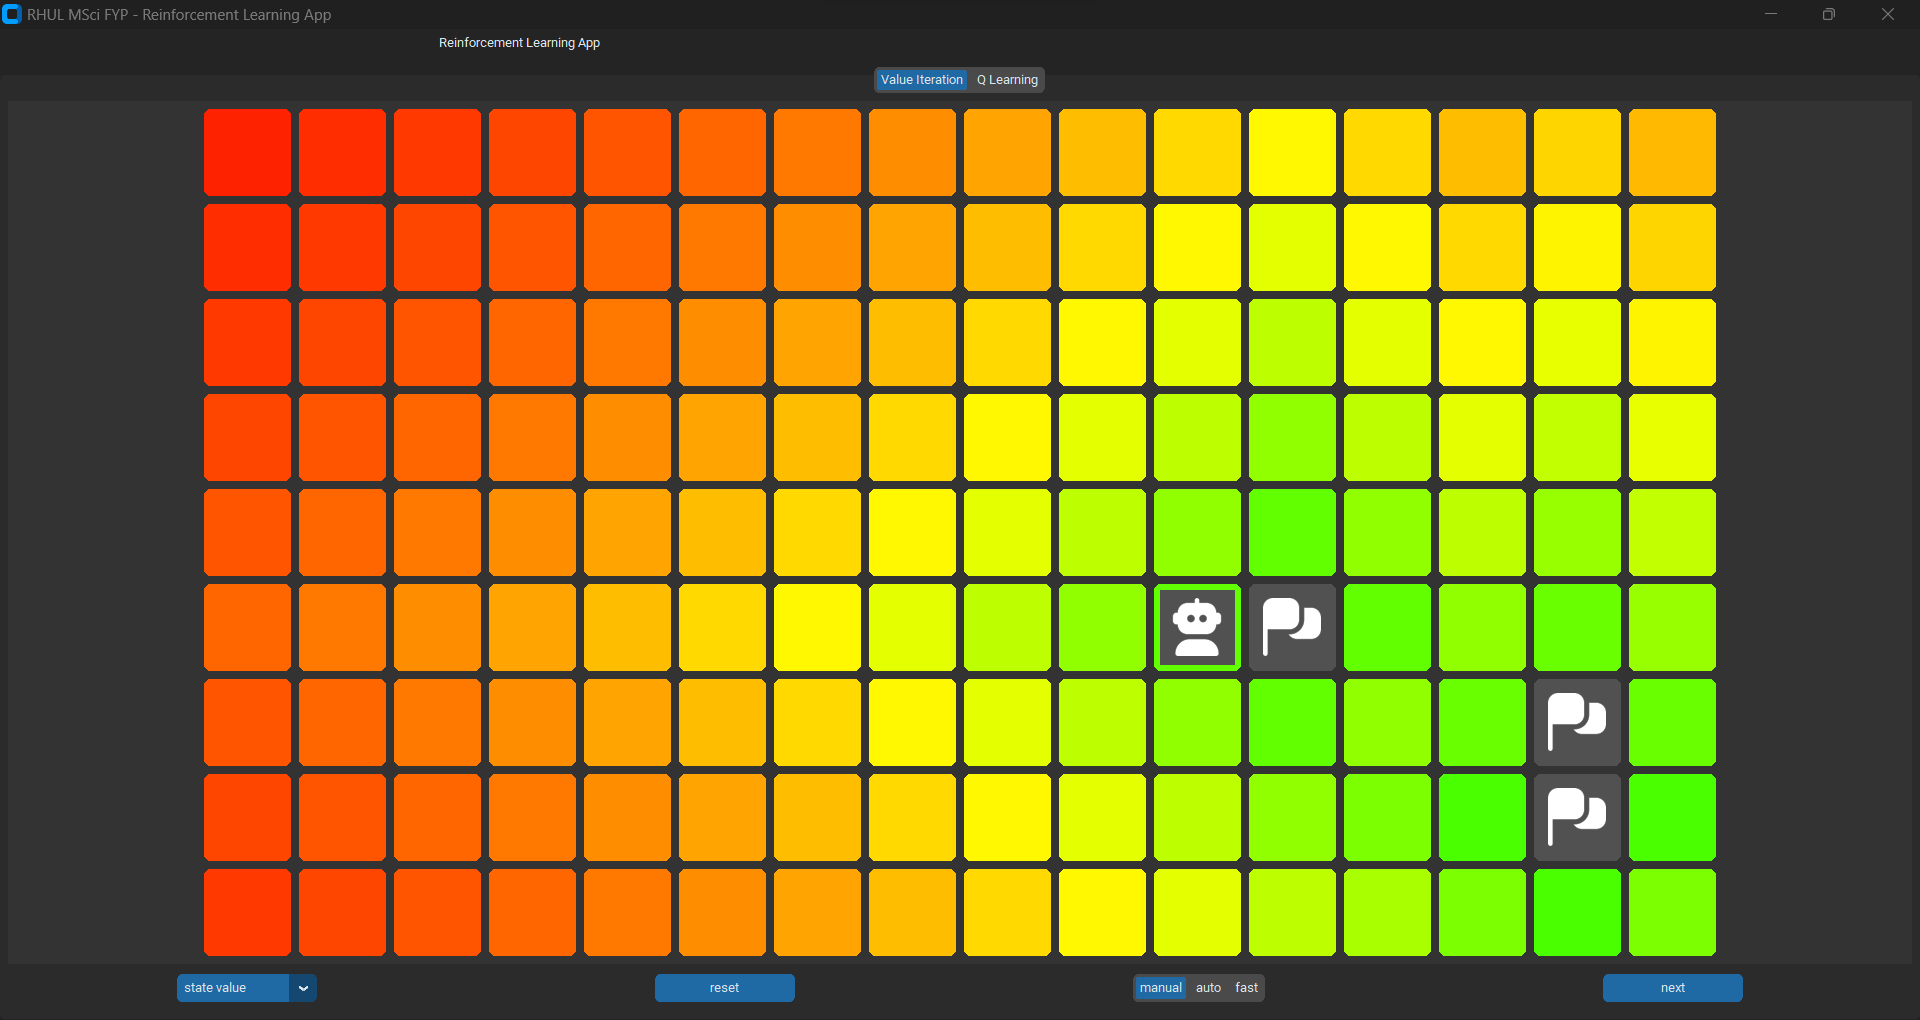
\includegraphics[width=0.95\linewidth]{state_value}
    \caption[width=0.5\linewidth]{\label{fig:screenshot:state-value-table} The V (state-value) table}
  \end{subfigure}%
  \begin{subfigure}{.5\textwidth}
    \centering
    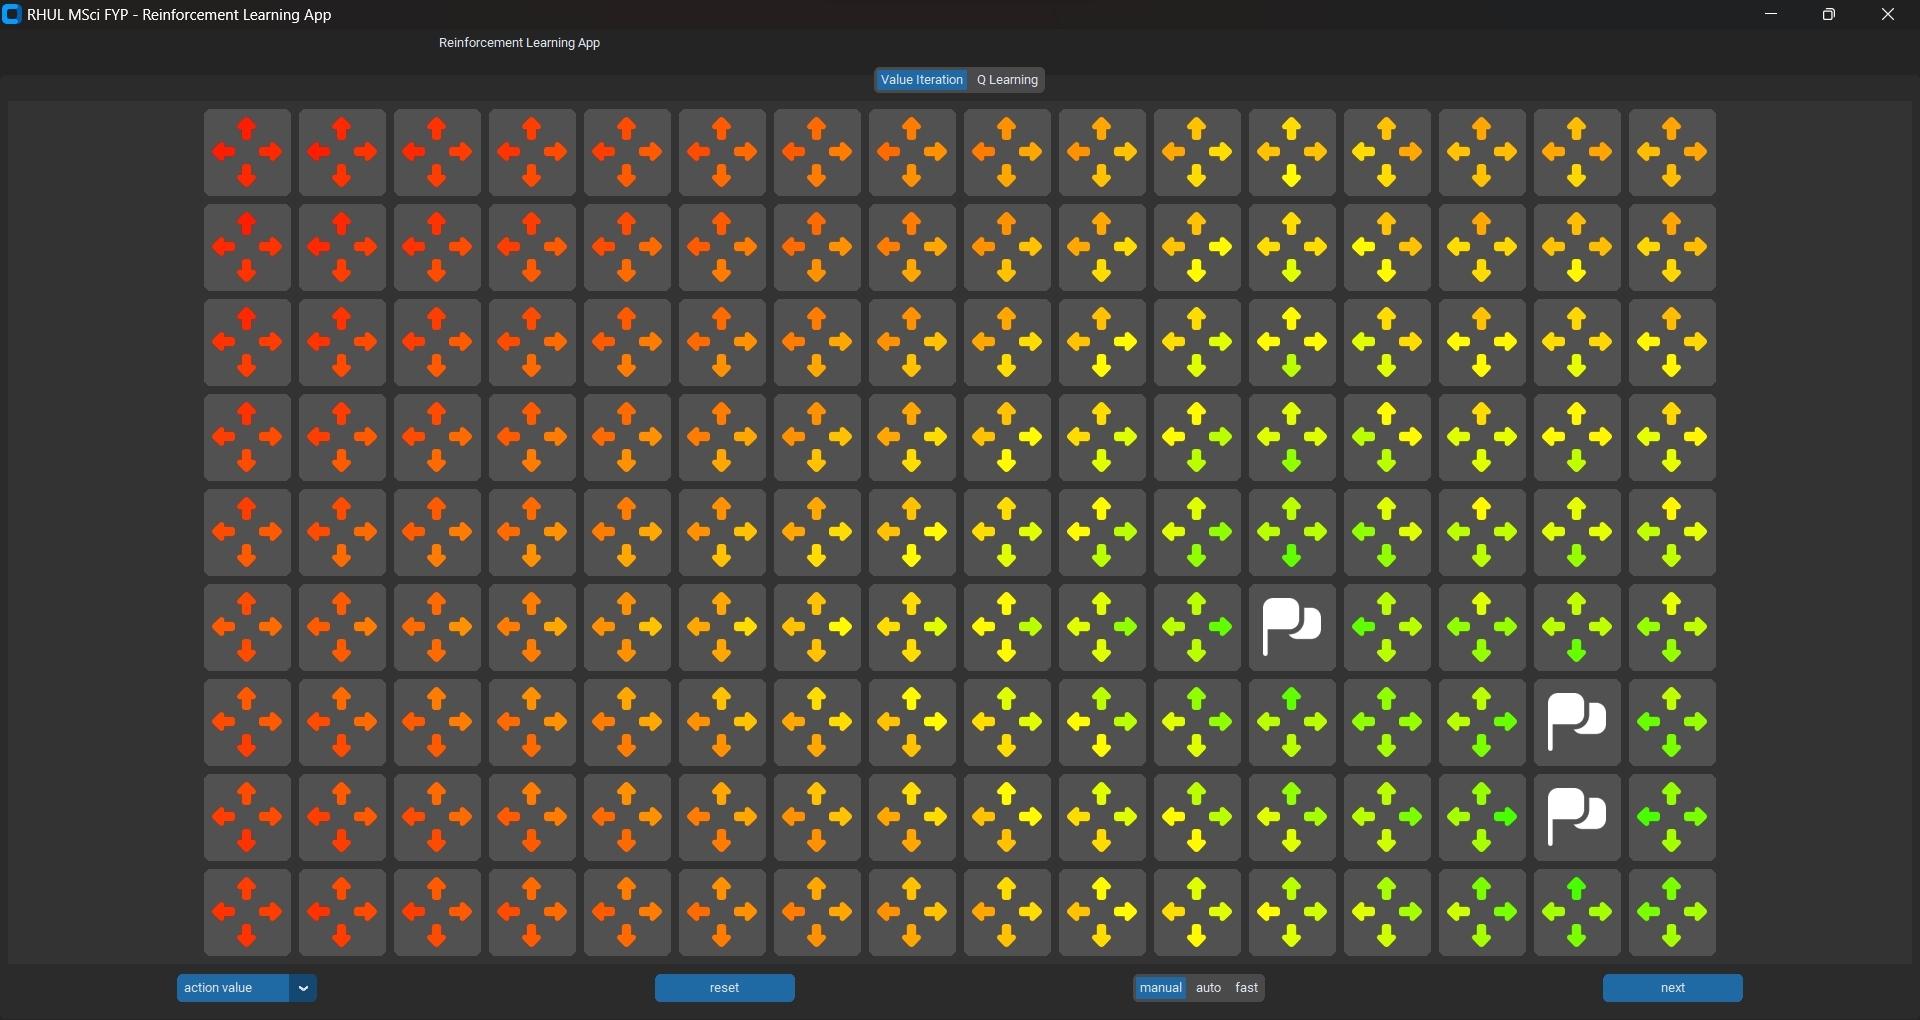
\includegraphics[width=0.95\linewidth]{action_value}
    \caption[width=0.5\linewidth]{\label{fig:screenshot:action-value-table} The Q (action-value) table}
  \end{subfigure}
  \caption{Two of the application's visualisations}
  \label{fig:app-ui}
\end{figure}

This chapter details the software engineering of the project and demonstrates how this allowed the project to succeed. Software engineering consists of methods and techniques to develop large and robust applications~\cite{van2008software}. Software engineering techniques are principally aimed at managing complexity and evolving requirements. As functionality and complexity have grown, the software engineering consideration of this chapter has become crucial. At the time of writing, the application has over 5,300 lines of Python code across 150 files.

A video of the application running can be accessed here:\\
\url{https://www.youtube.com/watch?v=yZL6JylAYhA}

\section{System Design}\label{section:system-design}

This application is written in Python with the model-view-controller architecture. Python was chosen for many reasons, such as its robust ecosystem of machine learning libraries, which are widespread and crucial for performant deep reinforcement learning in Python. Python is also a high-level language that is clear and readable. However, python has notable constraints. The predominant Python interpreter, CPython, is substantially slower than other implementations~\cite{pythonMachineLearning}. For compatibility, I have chosen this interpreter. To mitigate the effects in the most performance-sensitive areas of the application, I have used libraries such as Numpy, Numba, and Pillow, which allow me to move the bulk of the computation out of Python.  

The application has a complex GUI with controls that visualise the state of more complex reinforcement models. The model-view-controller architecture is well suited for this application's requirements, as it helps to reduce the coupling between these two different but connected modules. This reduced coupling has proved invaluable as I needed to change the GUI library several times to meet my requirements. Due to the nature of modern GUI frameworks, the code traditionally considered the view receives update signals from the user. For this reason, this project requires the use of the layered MVC pattern~\cite{webMVC,gamesMVC}, where the controller acts as a bridge between the model and the view. This is similar to the MVVM and MVP architectures~\cite{mvvm}.

\newpage
Multiprocessing is a method used to enable parallelisation. This is used in the application to allow the model to perform expensive computations without blocking the view. To the user, this means the application remains responsive at all times. Furthermore, this parallelisation allows the program to use the available hardware more effectively, thereby allowing tasks to be completed sooner. Unfortunately, multithreading could not be used for this task since Python implements a global interpreter lock (GIL). This lock prevents an interpreter from executing Python code in parallel. 

With multiprocessing, the program operates across multiple processes, each with its own address space. This separation presents an important challenge; for the program to work as one, it must communicate between these processes. This is called inter-process communication~(\ref{section:technical-decsions}). Managing communication effectively is vital to avoid race conditions. The MVC architecture provided a clean interface where the controller is responsible for transferring communications. At this boundary, to avoid race conditions, I use a request/response model where requests are queued and validated before being applied. On the response side, the model is considered a source of truth, and the view represents the most recent snapshot available.  

The application has been written in an object-oriented fashion with modern software engineering principles in mind~\cite{van2008software}. Object-oriented code is a programming paradigm built around the idea of combining state and functionality into one entity called an object. The goal of object-oriented code in this project and software engineering is to reduce coupling and increase cohesion. Coupling describes how interrelated different objects are, while cohesion describes how related code is within the same object. This application achieves low coupling and high cohesion by adhering to software engineering principles~\cite{softwareEngineringPrinciples} and using software design patterns where applicable.

Figure~\ref{fig:package-diagram} shows the overall structure of the application. While this diagram omits some details, it includes all the essential components. Starting from the top, the core of the model is the top-level entities, which consist of the agents, environments, and statistics. These core components together form a simulation. The learning system takes in the configuration the view provides and sets up the primary simulation with these options. The learning system also performs other operations, such as compiling the primary simulation's current state into a format useful to the view. The hyperparameter system runs multiple simulations with different hyperparameter configurations and records their results. Like the learning system, the hyperparameter package provides real-time feedback and results to the view. The hyperparameter system and learning systems each have their own data formats and update independently. For these reasons, the controller and communication channels have been separated. 

In the middle of the figure~\ref{fig:package-diagram}, the controllers connect the view and model with two bridges for bidirectional communication. The controllers also validate the requests and transform them into the actions performed on the model. Finally, at the bottom is the view; packages such as the state display create a view from the current snapshot of the model's state for the user to see. The UI controls package not only represents the current state, but with the user's action, they can trigger new requests. The statistics package contains the functionality for displaying simulation results, such as the reward history and hyperparameter tuning. The graphing package contains a framework for embedding graphs in the application in a way that allows them to fit in with the theme and enables exporting to PDF with a file picker.

\begin{figure}[H]
  \centering
  
  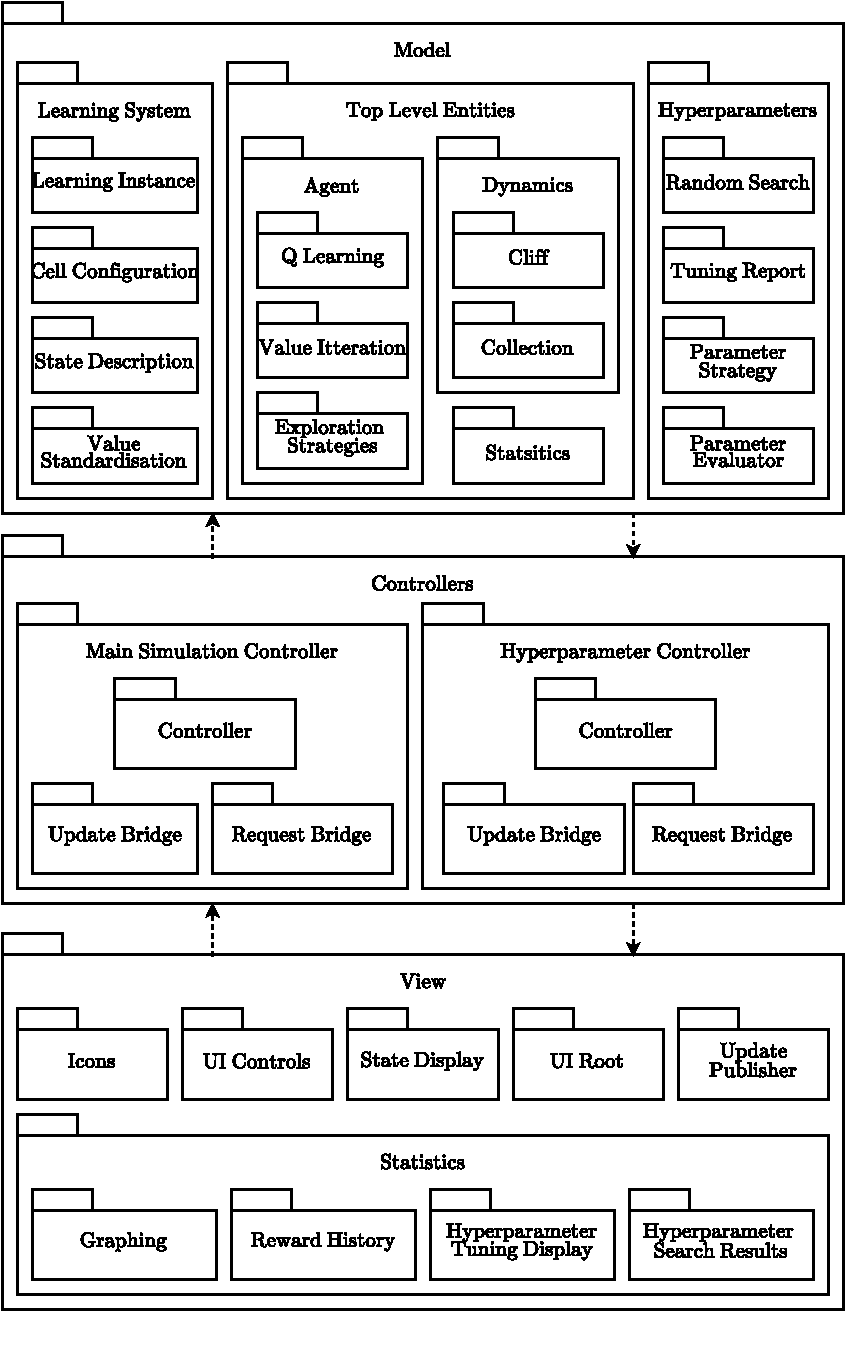
\includegraphics[width=\textwidth]{package_diagram-2.pdf}
  
  \caption{\label{fig:package-diagram} UML package digram of core packages from the application}
\end{figure}

\section{Technical Decisions}\label{section:technical-decsions}

Software development is made up of a large number of technical decisions. Most decisions are small and have a limited scope and consequences. In this section, I would like to highlight some of the key decisions and their impact on the project. Which algorithms to analyse is central to the project and sets the direction as a whole since it is the foundation upon which the rest of this project is based. Within reinforcement learning, there is a wide variety of available algorithms. These can widely be grouped into two main categories: tabular and function approximation. Of the latter category, there is deep refinement learning, one of the most cutting-edge areas of reinforcement learning research and where some of RL's biggest success stories and practical applications lie. 

Deep reinforcement learning is the application of deep neural networks to reinforcement learning, which can be applied in many ways, such as state representation or function approximation of value functions. While running these models can be straightforward, training them can be challenging. The cutting-edge models are trained using custom hardware at an immense cost~\cite{DeepRLCost}. While this project would not operate at that scale, even a modest network requires substantially more computation than a tabular method. Secondly, hyperparameter tuning is a significant challenge to these models~\cite{deepRLChallanges}. When slow iterations are combined with a difficult search, it can be severely time-consuming. This high startup cost can be mitigated partly by building upon others' work, but this is not the direction in which I wanted to take this project. With the potential risks of DRL, I chose tabular methods, allowing for an expansion of the scope in other directions.

Of the tabular methods, Value-Iteration and Q-learning have been implemented. Value iteration is a dynamic programming technique that efficiently solves the Bellman equations. Value iteration is an ideal starting point since it provides a baseline to measure other algorithms. Implementing Q-learning is essential because it is a practical algorithm and the basis of a lot of work in RL. Secondly, Q-learning is off-policy, allowing for different exploration strategies to be used while learning the optimal policy. This allows more flexibility and control in how the agent explores, and it is these exploration strategies that this project aims to analyse.  

As discussed in the system design section~(\ref{section:system-design}), the program requires a multiprocessing architecture to maintain a responsive user interface. Consequently, the application needs inter-process communication (IPC). This IPC forms the backbone of the application, so managing what and how to communicate has wide-reaching implications. Many IPC mechanisms are available to Python applications, such as signals, message queues, and shared memory. Shared memory allows two different processes to access the same memory at the same time. This can be performant, but if not managed effectively, there may be many ways that new functionality can lead to race conditions. Signals can be used to avoid race conditions by blocking processes from accessing the same resources simultaneously. Due to these concerns, I decided not to directly use shared memory in my application. However, I do use shared values where appropriate. Shared values are used to build up the hyperparameter reports between the worker processes. Shared values are a managed alternative to shared memory provided by Python. These managed objects, like shared values and queues, help avoid some of the pitfalls of multiprocessing. Nevertheless, these managed objects have a performance and latency overhead. 
\newpage

The link between the primary model and view processes is the most critical across the application because the user will directly experience any latency. Furthermore, if this connection were severed, the program might not be able to recover; for instance, it is used to signal a graceful shutdown. With these concerns, I found that the built-in solutions were not appropriate due to their relatively large overhead and latency. Instead, I have chosen the ZeroMQ messaging library because of its focus on low-latency communication and its fantastic reputation. Many large companies use ZeroMQ, it has a large community and is very stable. With this stability, I feel confident I can use it to build the backbone of the application. Like the inbuilt queue, ZeroMQ provides IPC with a message queue; however, unlike the inbuilt option, it does so without a message broker.  ZeroMQ's improved performance is partially due to its lack of a message broker. This lack of a message broker is what the zero in its name stands for.

There are many IPC styles however, they typically are broken into two main categories: memory sharing and message passing. While other parts of the application use the former, between the model and view I opted for the latter with the actor-model architecture. With this architecture, I could avoid lock-based synchronisation and utilise busy waiting. I chose to use two publish-subscribe channels for each topic, one for each direction. At initiation, each channel's details are negotiated with traditional IPC. I chose to use this dual pub-sub architecture as it allows unsolicited communication, unlike the Request-reply (Remote procedure call) pattern. These unsolicited messages allow the model to provide updates continuously as the model changes, such as providing constant feedback on the progress of the hyperparameter processes. 

When communicating messages between processes, the data should be concise while still allowing the receiver to interpret the message in the same way that the sender intended. This process is called serialisation, and it is crucial since it directly influences the work necessary for IPC. One interchange format used is textual, with XML and JSON being common choices. However, textual formats are not particularly efficient, especially for numerical data. So, instead, I chose a binary serialisation format since the application predominantly transfers boolean and numerical values. Since both endpoints are Python based and trusted, I could use the standard pickle module for serialisation. This module is ideal for our application since it is flexible, allowing the interchange format to be extensible rather than using some fixed or custom option. 

When serialising messages, compression should be a key consideration. Compression allows data to be reduced in size; this is done in two fashions: lossy and lossless. In lossy compression, uninformative, redundant or useless information is removed; however, this risks reducing the quality as well as size. A candidate for lossy compression would be the floating point values transferred since they rarely use the complete precision or range available. However, I have chosen to stick with a standard format for simplicity. Otherwise, due to the nature of the data of this application, there isn't any real opportunity for lossy compression. Lossless compression involves identifying patterns in data and representing these more concisely. This process could be used with this application's data. However, I have chosen not to use lossless compression since the size of messages is so small the lossless compression overheads are not worth the gains. 

\newpage
\section{Workflow}


All aspects of this project are stored under the Git version control system, and changes made on this project are grouped into small units called commits. Each commit belongs to a branch and has a message summarising the changes. Conventional commits~\cite{conventionalCommitsOnline} is a standard for commit messages. In this project, I have followed this standard because it keeps the commit message consistent and enables the use of tools such as automated change log generation and versioning. As this project has a single author, I have chosen to use branches to group related work together instead of following a specific branching strategy. However, like most branching strategies, the main branch represents the project after each stage of work is finalised. Therefore, this branch is always in a complete and functional state without blocking partial work. 

One essential part of this project and its workflow is documentation. The documentation is written alongside the code in what are called docstrings. This serves many purposes. Firstly, the co-location helps keep the documentation in sync with the application. Special linting rules ensure that these docstrings are written consistently for every piece of code, guaranteeing 100\% documentation coverage. Docstrings are also integrated into the Python language with the `help` command, and most editors integrate docstrings so they are accessible during development. Importantly, this documentation is made accessible as a documentation site. This site is generated automatically for these docstrings and other aspects of the code. This process results in a searchable, linked documentation page that is up-to-date~\cite{pythonAutoDoc} and covers all of the code. 

Testing is integral to this project. As part of my workflow, I write unit tests. Unit tests are pieces of code that perform validation and verification parts of the main application. A unit testing framework has been configured to run these tests and collate the results. All tests must pass before each commit can be made, which means that regressions are spotted quickly. These tests are also integrated into the IDE to provide increased feedback and ease of debugging. While testing can be valuable, it can be costly. Daka et al. found developers spent a substantial amount of time writing tests~\cite{unitTestingSurvey}. The returns from testing can be especially low for trivial code that can take several times longer to test than create. For this reason, I have limited testing to the important and complex areas of the program.  

The development environment is the system of programs where this workflow takes place. This project is configured to work well with a particular Integrated development environment (IDE); for instance, the IDE will be able to start the application with a debugger attached, allowing the user to step through the code in the editor. Code quality is maintained in this repository with several automated tools. Static code analysis tools enforce a consistent code style and check for typing errors. I have configured these tools to integrate with the IDE, giving immediate feedback so issues can be addressed quickly. Furthermore, Git is configured with pre-commit hooks, so these tools must run and validate the code before every commit. Furthermore, these tools can be integrated with CI/CD pipelines, which is particularly useful for collaborative projects.

While all of the tooling for this project improves many aspects of development, this may be difficult to set up and provides many opportunities for discrepancies to emerge between different setups. For this reason, I have created a development container. This container fully specifies every tool and the version to be installed. This containerised environment makes it easy to set up the environment and consistent each time. Containers for development are rapidly growing in interest~\cite{developmentContainers}. 
\newpage
For the sake of consistency, the application itself has been configured with a dependency management and packaging tool. All of the libraries the application relies upon are specified in the standard `pyproject.toml`, and the tool manages their installation in an isolated virtual environment. This process makes it easy to distribute this application and avoids inconsistencies on different computers.


\section{Functionality and Usage}

The application's functionality revolves around running reinforcement learning simulations and allowing the user to interact with and analyse the effects of different options. These simulations encompass two main units: agent and dynamics. The agent unit encompasses the functionality for learning and decision making while the dynamics unit encompasses a grid world Markov decision process. These units are interchangeable and configurable by the user dynamically through controls in the user interface and through a configuration file \path{config.toml}. The results of these learning experiments are expressed by the application in several ways, such as a state-by-state view, information displays, and graphs.


\subsection{Getting Started}

The project is set up as a standard distribution package, and poetry is the build backend. While you may also use poetry as the build front-end if you have it installed, it may be excessive if you are only interested in starting the application.

Pipx is a simple build frontend that should be familiar to you if you have experience with pip. Instructions on how to install Pipx for your platform can be found \href{https://pipx.pypa.io/stable/installation/}{here}. Once you have installed pipx, the application can be started with the following command:
\begin{verbatim}
python3 -m pipx run --spec . start
\end{verbatim}
This command will take longer than usual for the first run as pipx sets up the application. You can find more information about this application and how to start it in the \say{readme} file in the code folder.
\newpage
\subsection{User Interface}

The user interface is not only a significant component of the project's functionality but also the user's window into the entire application. When starting the application, you are greeted by a window composed of three main sections stacked vertically. At the top, there is a section that contains the main controls. These controls select the most significant options of the primary simulation, such as the agent and dynamics. If the agent is off-policy, you can select its own exploration strategy. There is also a reset button that will reset the agent's knowledge and, therefore its policy.

In the middle, there is a tabbed area. The first tab is the primary display, which visualises the current state of the main simulation. The second tab displays the reward history of the simulation as a graph. The third and fourth tabs can run auxiliary simulations in the background to examine the effect of different hyperparameter choices. The third tab shows graphs of the effects of varying each hyperparameter and the reward achieved with 95\% confidence bounds. All graphs in the application have an option to save their contents as a portable document file. Once pressed, this save button will allow the user to provide where to save this graph. Finally, the fourth tab controls a random search procedure. The start/stop button controls this procedure. When running this system searches for the best parameter choices to minimise regret~(\ref{section:measuring-performance}).

The main display on the first tab visualises the current state of the primary simulation. All of the environments that are implemented currently are based around a grid world. The display visualises this grid world with a corresponding grid of cells, each cell representing a possible position the agent can occupy. The function of this grid will vary based on the display mode. In the initial (default) display mode, a robot icon represents the agent's location, flags represent the agent's goals and stop icons represent obstacles. In other display modes, arrows represent the agent's actions in each state and a colour scale is used to represent the agent's interpretation of value. On this colour scale, hues vary from red to green, where red is the least valuable state and green is the most valuable state or state-action.

At the bottom are specific controls specific to the primary simulation and visualisation. There are controls for selecting the display mode and allowing the user to step through the simulation manually or automatically. In this section there is also a secondary reset button, this button resets the current state of the agent to the initial state for the episode. Unlike the reset button at the top of the application, the agent will retain its knowledge.


\begin{figure}[H]
  \centering
  
  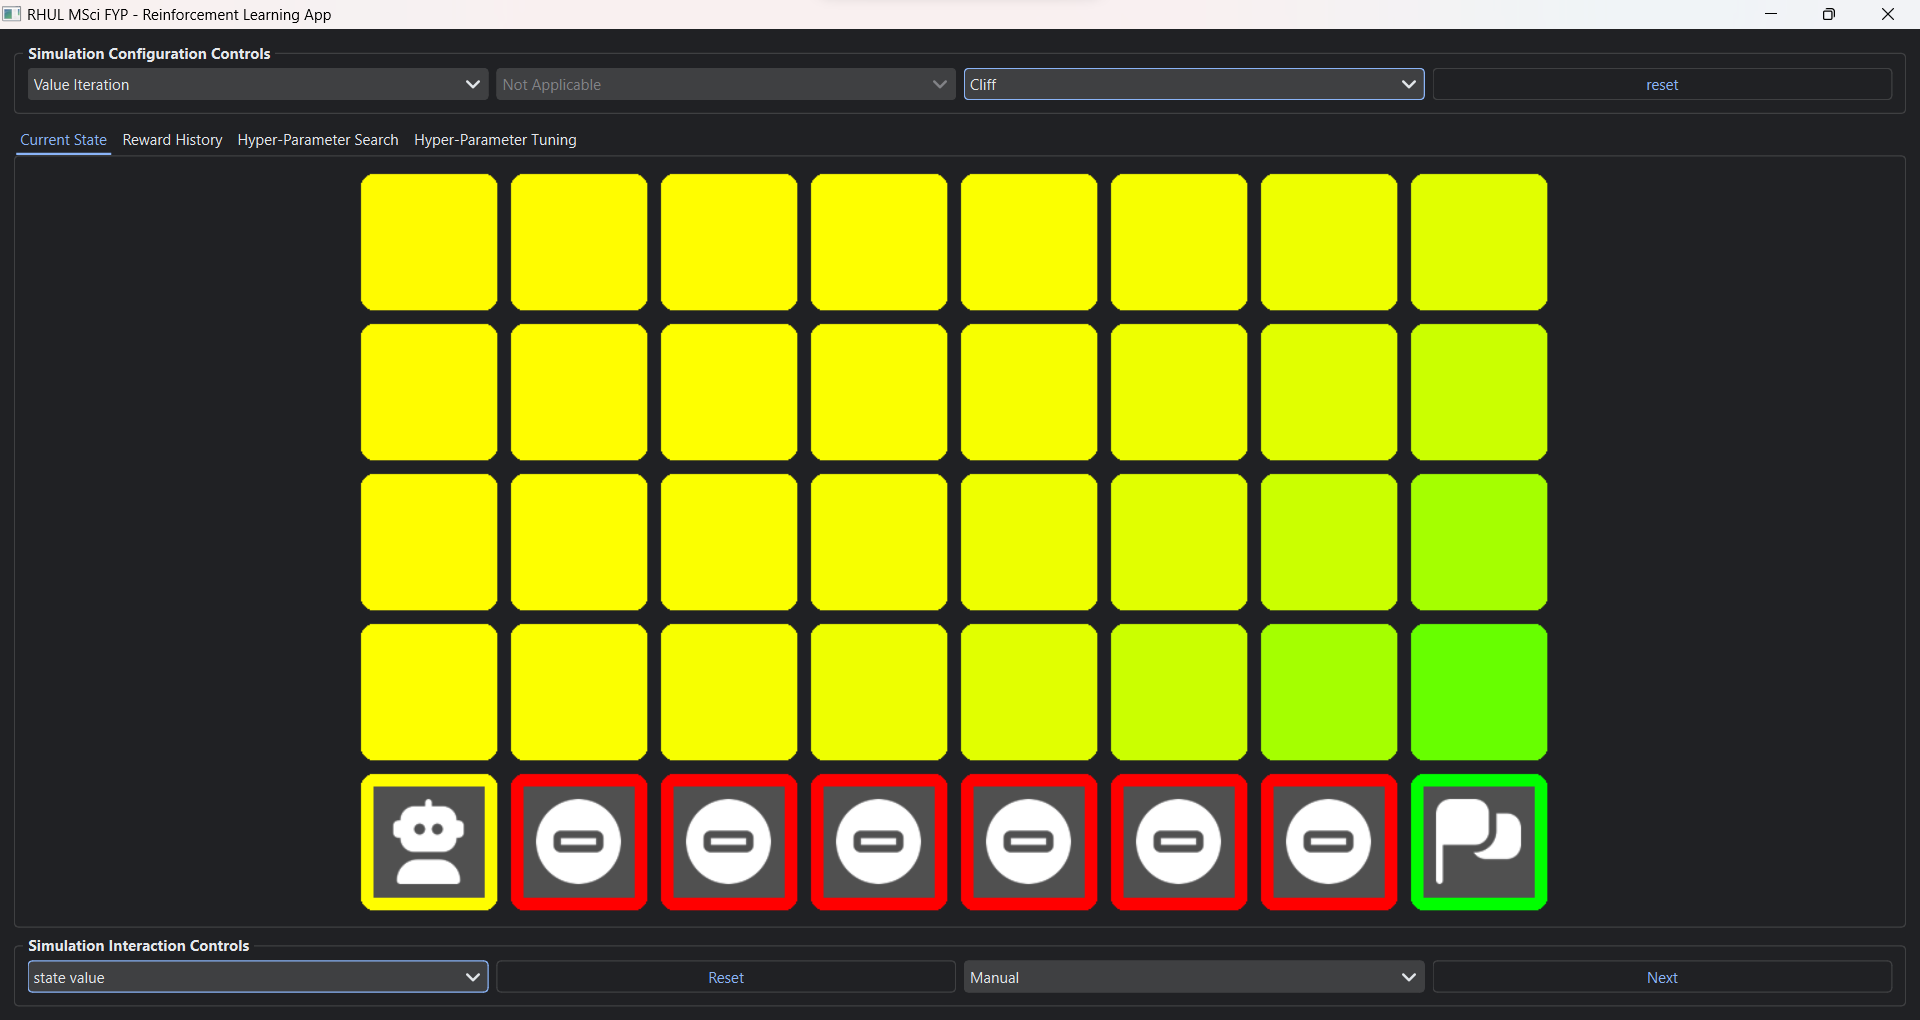
\includegraphics[trim={0 0 0 6mm},clip,width=\textwidth]{ui-screenshots/state-value-2.png}
  
  \caption{\label{fig:screenshot:current-state} "Current State" tab with optimal state-value visualisation of the cliff environment}
\end{figure}

\begin{figure}[H]
  \centering
  
  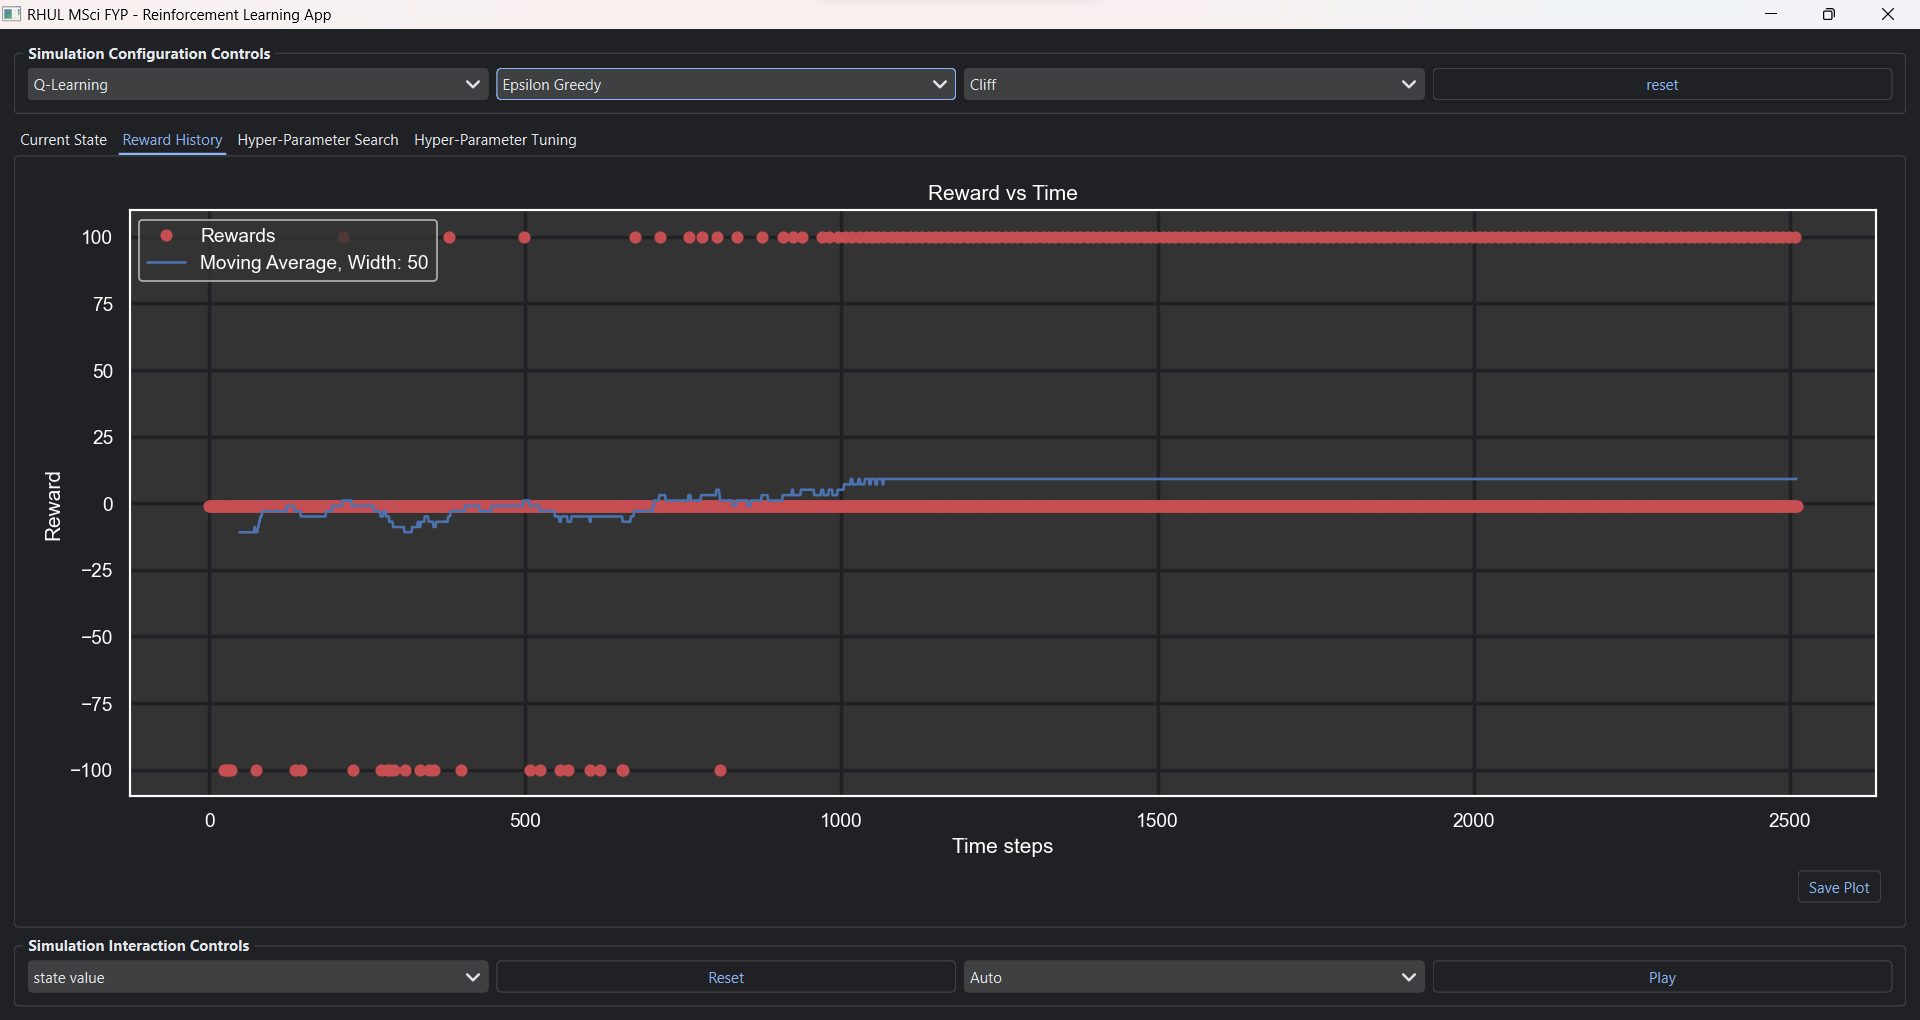
\includegraphics[trim={0 0 0 6mm},clip,width=\textwidth]{ui-screenshots/reward-history.png}
  
  \caption{\label{fig:screenshot:current-state} "Reward history" tab with Q-learning agent in the cliff environment}
\end{figure}

\begin{figure}[H]
  \centering
  
  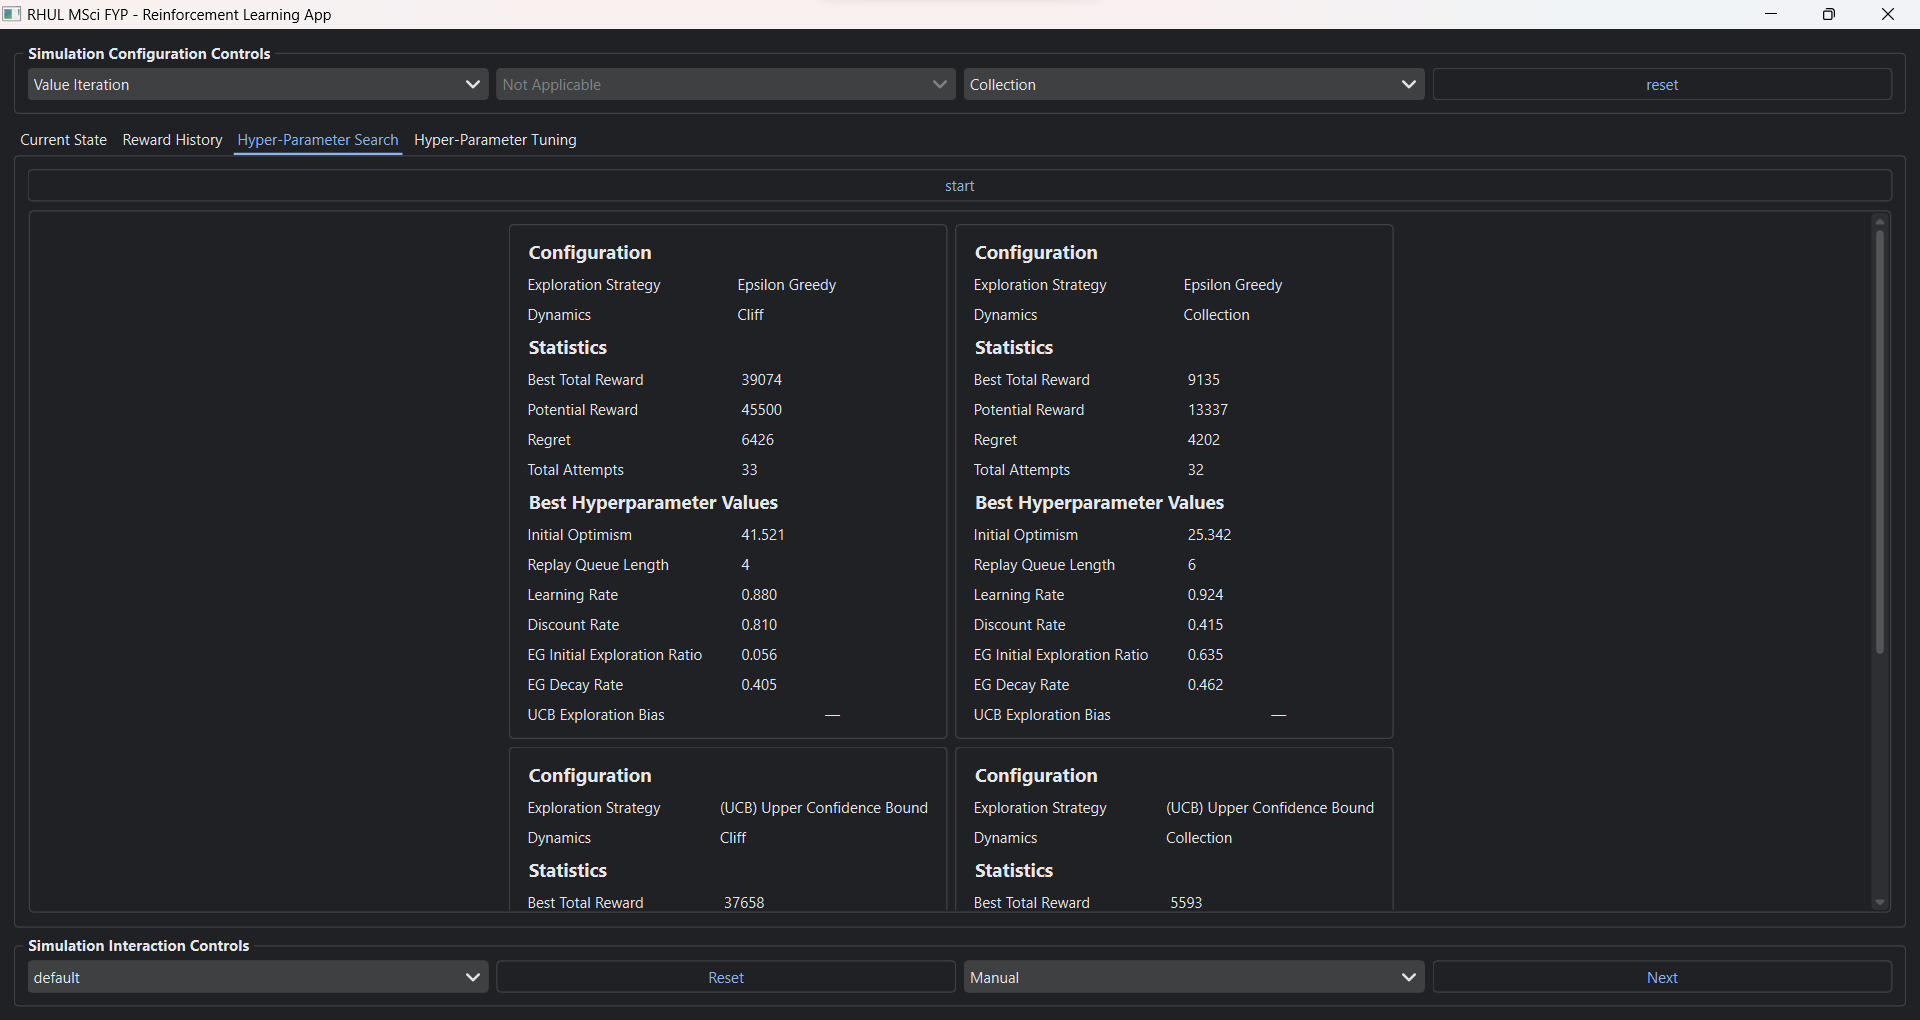
\includegraphics[trim={0 0 0 6mm},clip,width=\textwidth]{ui-screenshots/random-search.png}
  
  \caption{\label{fig:screenshot:current-state} "Hyper-parameter Search" tab showing search results}
\end{figure}


\begin{figure}[H]
  \centering
  
  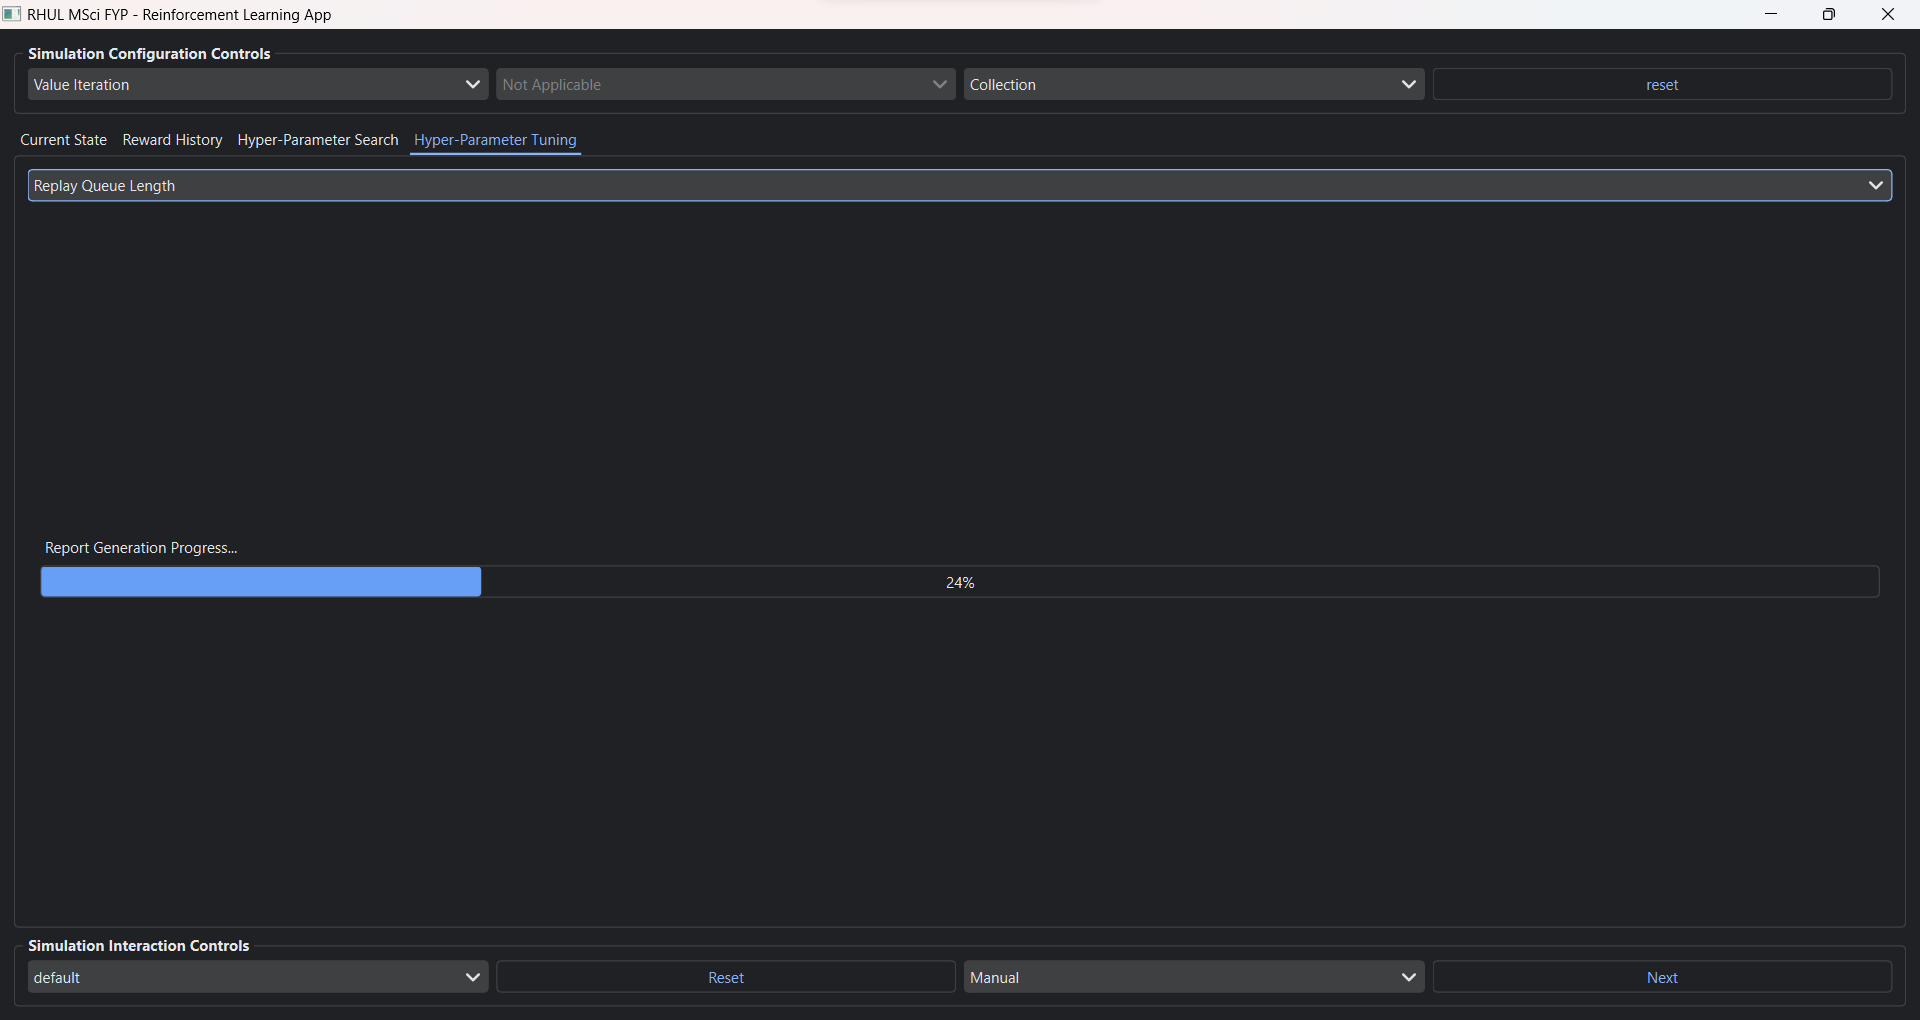
\includegraphics[trim={0 0 0 6mm},clip,width=\textwidth]{ui-screenshots/loading-screen.png}
  
  \caption{\label{fig:screenshot:current-state} "Hyper-parameter Tuning" tab loading screen}
\end{figure}

\begin{figure}[H]
  \centering
  
  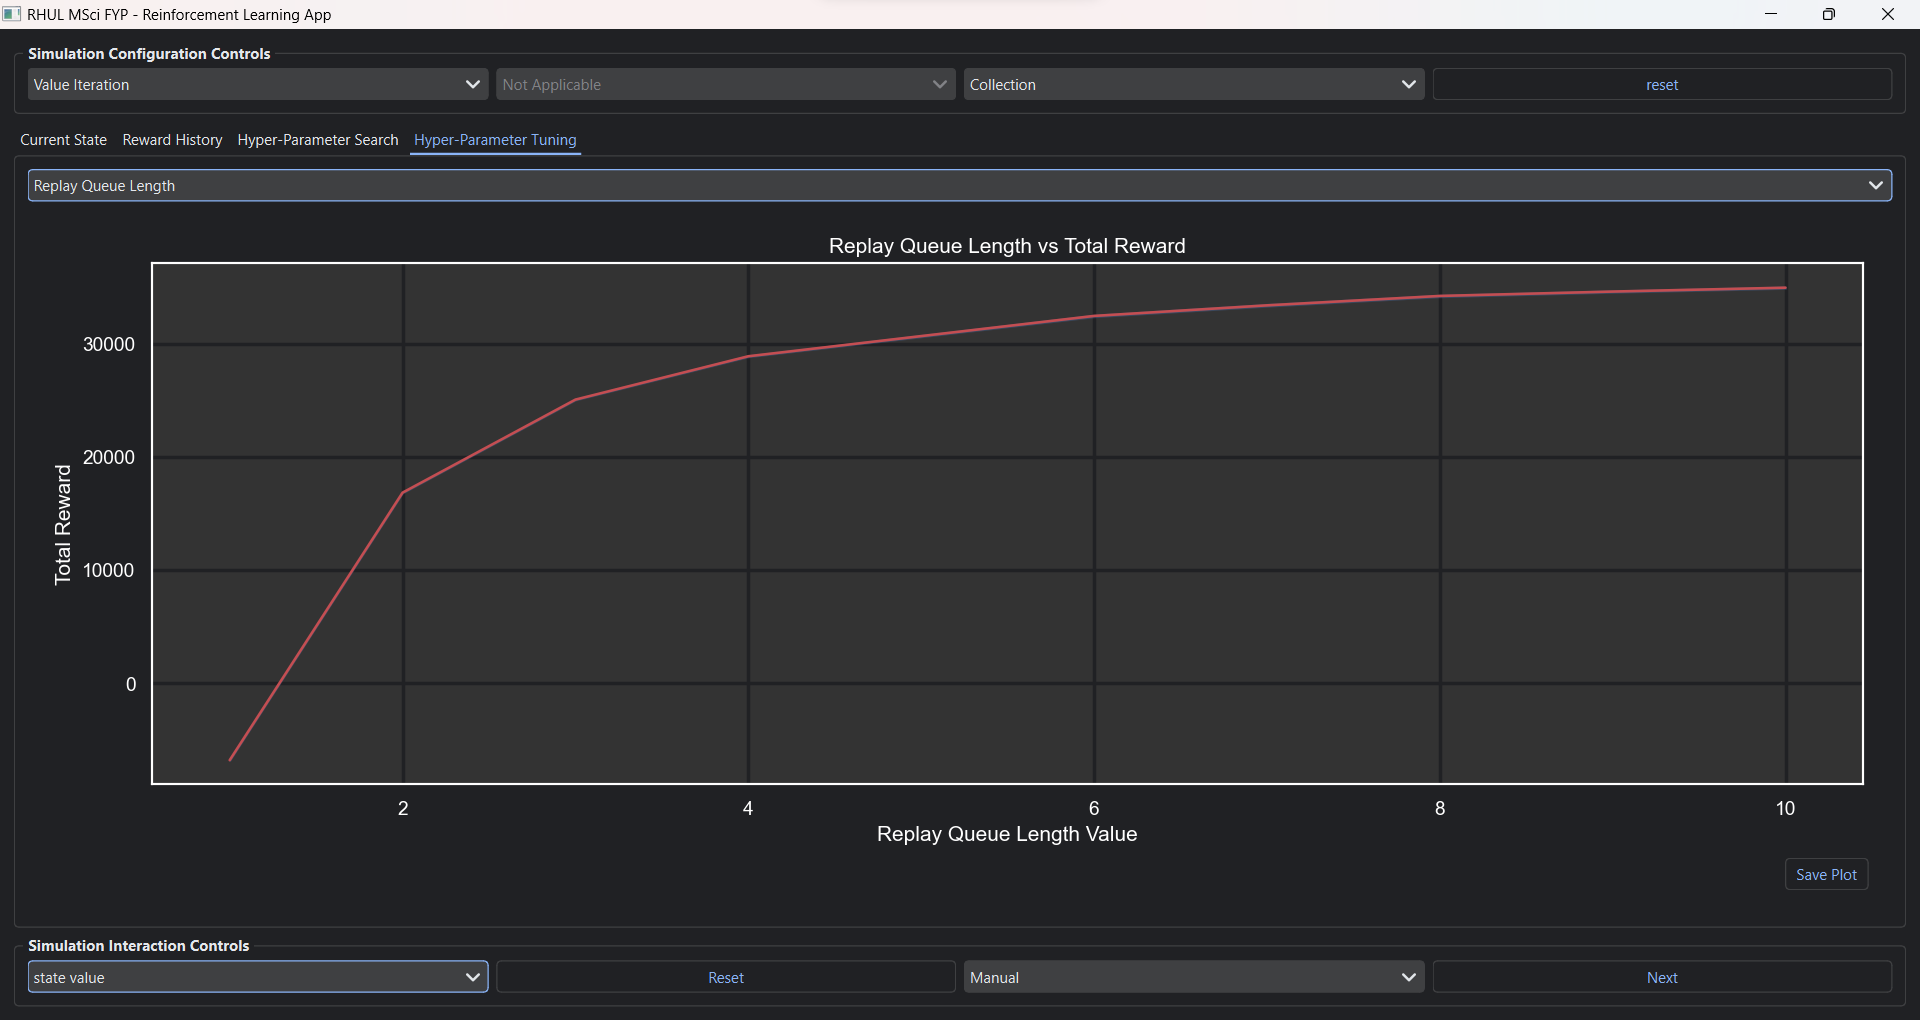
\includegraphics[trim={0 0 0 6mm},clip,width=\textwidth]{ui-screenshots/hyper-tuning.png}
  
  \caption{\label{fig:screenshot:current-state} "Hyper-parameter Tuning" tab showing the results of tuning the reward queue length}
\end{figure}


\chapter{Exploration Strategy Effectiveness}
\label{chap:exploration-strategy-effectiveness}
Q-learning is an off-policy process, which means that the policy that the policy that it is learning and improving is not necessarily the same as the policy it is following during exploration. By this, the actions chosen by a Q-learning agent may be independent of its current beliefs of the values of each action. Off-policy learning has several advantages, such as the fact that it may explore the environment more fairly and thoroughly than an on-policy approach. An on-policy approach may be incentivised to explore thoroughly if its initial estimates are particularly optimistic. However, in a stochastic environment where rewards are random with a large degree of spread, it may still be difficult for an on-policy technique to properly assess the rewards before falling into an in-optimal pattern.  

On-policy reinforcement learning algorithms such as SARSA do have many advantages in deep reinforcement learning (DRL). In DRL, a deep artificial neural network is used to estimate the Q-values~\cite{deepRLOverview}. DRL can help generalise reinforcement learning to larger state spaces than is possible with tabular methods. Typically, in this context, fully off-policy methods do not perform as well as on-policy or hybrid methods~\cite{deepOnVsOffPolicy} since off-policy methods suffer from instability\cite{sutton2018reinforcement}.

In this project, I have focused on the off-policy Q-learning method. This chapter details the performance and effects of different exploration strategies. An exploration strategy is the policy that the agent follows during training as opposed to the learnt policy. This exploration strategy may be any method to select an action; however, to maintain the guarantees of convergence, this policy must reach all states infinitely often~(\ref{section:impl-conditions}). While a random action section, a random walk, does meet the convergence criteria, it is inefficient in terms of rewards received or information gained. As an improvement in these measures, more sophisticated strategies have been developed that take into account many factors.

\newpage
\section{\texorpdfstring{$\varepsilon$}{Lg}-Greedy}

\begin{figure}[H]
  \centering
  
  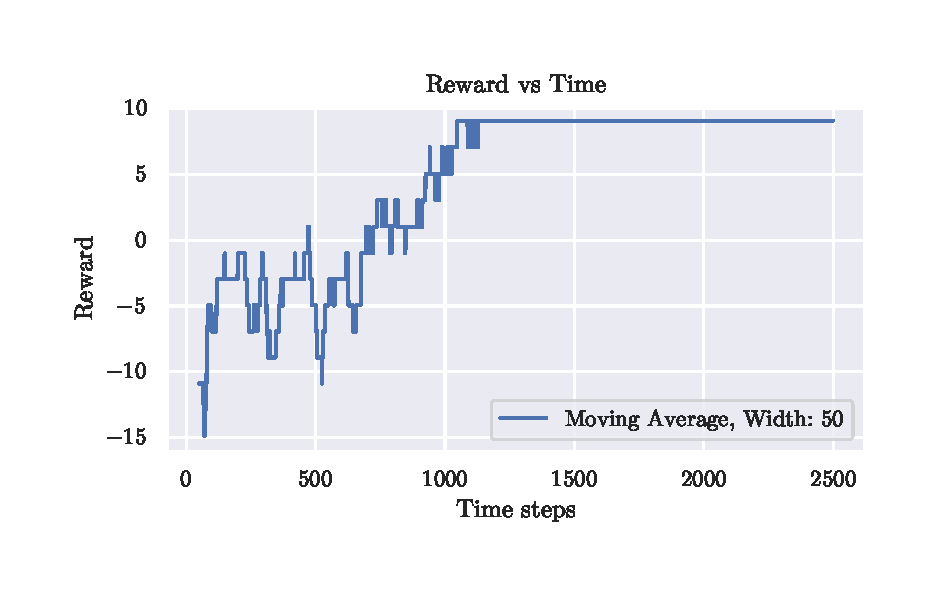
\includegraphics[trim={0 1cm 0 1cm},clip,width=\textwidth]{reward-history/EG.pdf}
  
  \caption{\label{fig:reward-history:eg} Reward history for an $\varepsilon$-Greedy exploration strategy instance}
\end{figure}


The $\varepsilon$-Greedy is the most straightforward strategy implemented in this project, and it acts as a good baseline. In its basic form, a parameter $\varepsilon$ controls the probability of the agent acting in two modes. The first and typically most common mode is where the agent selects the best action based on the current Q-estimates. In this first mode, the agent is essentially operating in an on-policy manner. In the second mode, the agent selects an action at random~\ref{section:impl-conditions}.

This epsilon parameter controls the ratio between the agent's exploration and exploitation. Having high exploitation can garner more rewards in the short term, but this has a considerable opportunity cost of not finding potentially lucrative strategies. On the other hand, if already following an optimal policy, an exploratory action would not be optimal, and in the case of the cliff environment, it can be potentially devastating. In the beginning, higher exploration may be necessary to avoid local minima, but higher exploitation can be more rewarding once the policy converges. To address these varying exploration-exploitation pressures, the $\varepsilon$ parameter can be dynamically adjusted during training. This project implements the traditional discounting with a fixed hyperparameter; however, more advanced reward-based techniques have been found to be successful~\cite{rewardEpsilonDecay}. My hypothesis is that decaying this learning rate with respect to the temporal difference errors may be more successful. 

Despite $\varepsilon$-Greedy's simplicity, figure~\ref{fig:reward-history:eg} shows how competitive this strategy can be when tuned to the environment. A combination of optimistic initial estimates and forced exploration can be extremely efficient. Unfortunately, to achieve these extraordinary results, each hyperparameter needs to be "just right" for the environment; this doesn't generalise easily and can be thought of as a form of over-fitting. I cover the effects of the exploration decay rate parameter in more detail in section~\ref{edgr-section}.


\section{Upper Confidence Bound}

\begin{figure}[H]
  \centering
  
  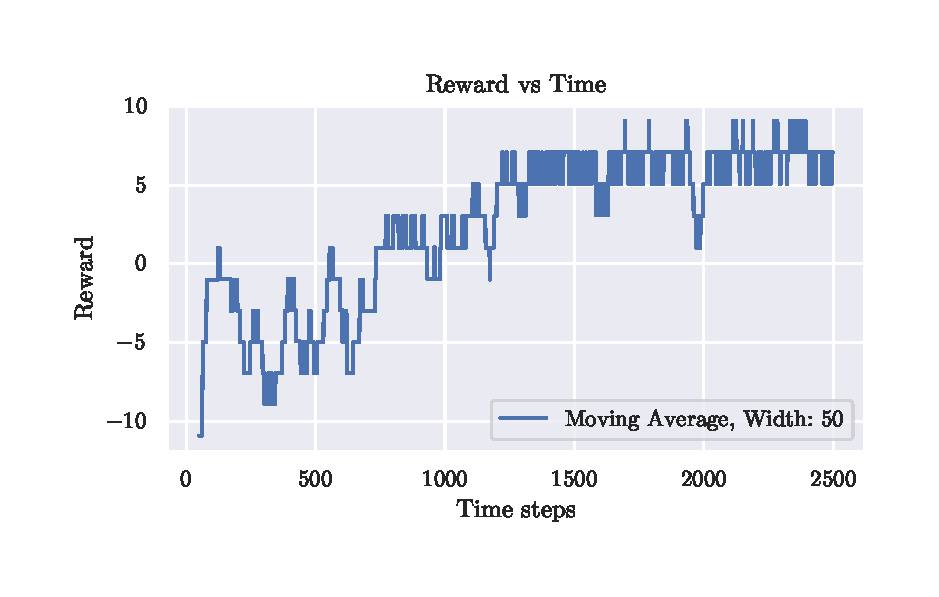
\includegraphics[trim={0 1cm 0 1cm},clip,width=\textwidth]{reward-history/UCB.pdf}
  
  \caption{\label{fig:reward-history:ucb} Reward history for an UCB exploration strategy instance}
\end{figure}


The upper confidence bound (UCB) exploration strategy uses the current Q value estimates to direct its decisions; however, instead of using randomness to dictate exploration, it uses an informed method. UCB prioritises actions that have the highest potential for reward. The potential value is determined from two factors: the current value estimate and a measure of confidence in the value estimate. The key idea behind this confidence measure is that it relates to the number of samples that have been made of the state action~\cite{sutton2018reinforcement}. This relationship is defined in the following rule:


\begin{equation}
  A_t \doteq \underset{a}{\operatorname{argmax}}\left [Q_t(a)+ c\sqrt{\frac{\ln t}{N_t(a)}} \ \right ]
  \label{eqn:ucb}
\end{equation}
~\cite{sutton2018reinforcement}

where $A_t$ represents the action chosen at time $t$, and $N_t(a)$ represents the number of samples of action $a$ have been taken at the current time. 

\begin{figure}[H]
  \centering
  
  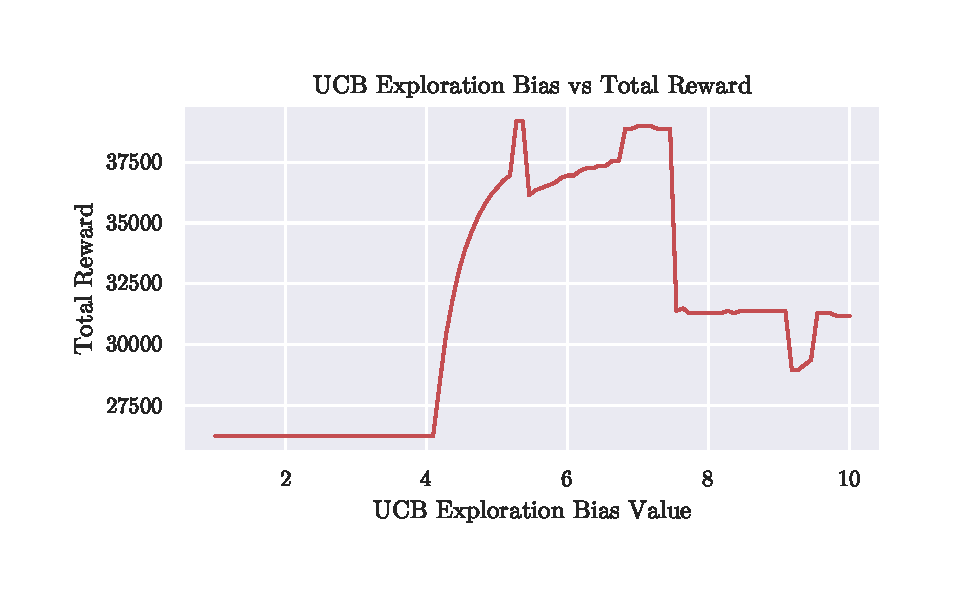
\includegraphics[trim={0 1cm 0 1cm},clip,width=\textwidth]{hyper-paramiters/ucb-exploration}
  
  \caption{\label{fig:ucb-exploration-bias}}
\end{figure}


In essence, this equation is optimistic as it will never underestimate or fail to explore an action. It also provides a natural balance between exploration and exploitation. Furthermore, Without a discount factor, this strategy naturally tapers off exploration over time. Instead of even exploration like $\varepsilon$-Greedy, UCB avoids redundant exploration in areas that have already been covered. However, UCB is not without hyper-parameters. $c$ controls the exploration balance; higher values encourage more exploration. Like $\varepsilon$ from $\varepsilon$-greedy, this parameter can have a profound impact on the strategy's performance. Figure~\ref{fig:ucb-exploration-bias} shows how a change in this balance can almost double the cumulative reward. 

Figure~\ref{fig:ucb-exploration-bias} also illustrate how the effects of $c$ can be both gradual and abrupt. This stems from the relationship between the agent and environment and how they are both deterministic. Generally, gradual improvement can be found when the agent makes slight changes in the amount of exploration, whereas abrupt changes happen if the agent discovers shortcuts or not.  From my experience, values $c<1$ operate in an on-policy fashion and $c>10$ over explore.

$\epsilon$ greedy is able to get extraordinary results at the cost of under-exploration. UCB risks the opposite issue; it may over-explore. This is a consequence of its uncertainty term~\ref{eqn:ucb}, it is optimistic and constantly growing; this guarantees the strategy will always explore enough to converge fully. Unfortunately, it is never completely done exploring. The $\ln t$ operator helps to mitigate this issue over time. However, at the beginning, the UCB is prone to re-exploring areas over new ones. I believe this behaviour explains some of the oscillations in figure~\ref{fig:reward-history:ucb}. In UCB's favour, it considers the estimated value in all of its exploration and has received the least penalty of any strategy.


\section{Model-Free Best Policy Identification}

\begin{figure}[H]
  \centering
  
  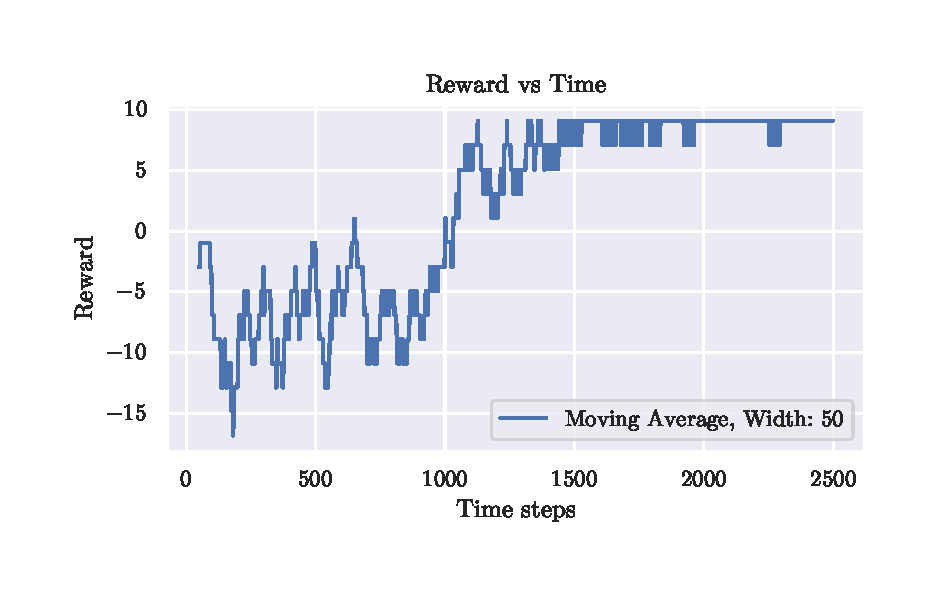
\includegraphics[trim={0 1cm 0 1cm},clip,width=\textwidth]{reward-history/MF-BPI.pdf}
  
  \caption{\label{fig:reward-history:mfbpi} Reward history for an MF-BPI exploration strategy instance}
\end{figure}


Model-Free Best Policy Identification (MF-BPI) is a state-of-the-art method that has demonstrated an improvement in exploration over its contemporaries, such as UCB~\cite{modelFree}. This exploration strategy optimises for the best policy identification that was introduced in section~\ref{bpi-introduction}. Unfortunately, the characteristic time $T^*$ metric is non-convex~\cite{characteristicTimeNonConvex} and requires extensive knowledge of the MDP's underlying distribution. Model-Free Best Policy Identification addresses both of these issues to make this approach practical.

This exploration strategy uses an allocation vector $\omega$ that distributes the search effort across the state-action space however instead of optimising this with respect to the characteristic time $T^*$ metric, they derive a new tight convex upper bound $\tilde{U}$. 

\begin{equation}
  \tilde{U}(\omega) \doteq \max_{s,a \neq \pi^\star(s)} \frac{H(s,a)}{\omega(s,a)} + \frac{H}{\min_{s'} \omega(s',\pi^\star(s'))}~\cite{modelFree} \label{eqn:upper-bound-def}
\end{equation}


This new metric overcomes the first challenge; however, in the equation~\ref{eqn:upper-bound-def}, it is evident that it is still dependent on the optimal policy and the optimal value function, something an agent would not have access to. Therefore to make this practical, the MF-BPI strategy estimates these values by maintaining an ensemble of value tables, from which it can estimate their variance. MF-BPI also uses a bootstrapping technique to ensure that its uncertainty decreases over time. Due to this bootstrapping, they claim that MF-BPI does not require forced exploration to ensure all state-action pairs are visited infinitely often; however, their implementations provided did include forced exploration, Garivier et al. said \say{the forced exploration step is rarely useful, but in some cases really necessary and not only for the theorems}~\cite{characteristicTime}

MF-BPI strategy requires three hyperparameters: the ensemble size, the exploration parameter and what I call error sensitivity. However, the strategy does not seem to require extensive tuning and performs well with the provided values. While this strategy has not performed quite as well as a perfectly tuned $\varepsilon$-greedy, it is nearly as good without any tuning. Notably, this strategy's regret is competitive despite not being the objective. This strategy was originally developed and tested for stochastic environments, I expect it might perform better under those conditions. Overall MF-BPI's performs well but its incredible generalisation is its most impressive characteristic. 


\section{Hyperparameter Selection}

\begin{figure}[H]
  \centering
  
  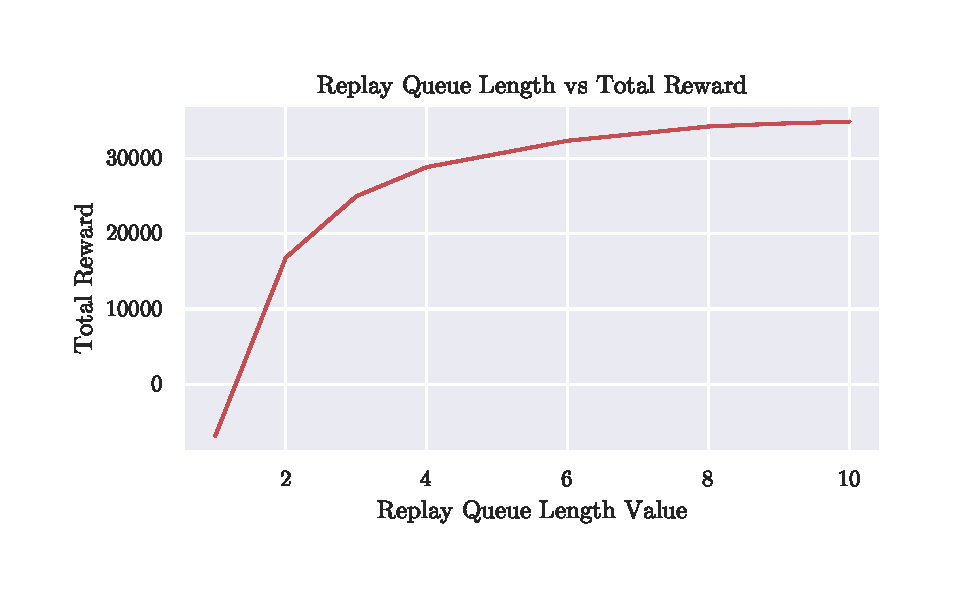
\includegraphics[trim={0 1cm 0 1cm},clip,width=\textwidth]{hyper-paramiters/replay-queue-length.pdf}
  
  \caption{\label{fig:replay-queue-length}}
\end{figure}

Q-learning itself and each exploration strategy require some parameters which are set outside of the learning process. Figure~\ref{fig:replay-queue-length} Demonstrates how hyper-parameter values can have a profound impact on the effectiveness of the agent. However, selecting the best parameters is not straightforward. The first difficulty is that the best parameter choice depends on both the agent and the environment that it operates in so they are not transferable and must be found through experimentation. The second difficulty is that the hyper-parameters are not independent; different choices may compound or interfere with each other. Finally, building on the second issue is the number of parameters. For Q-learning with $\varepsilon$-greedy, there are six tunable parameters, This makes visualising the whole hyper-parameter space impossible. 


For this reason, the application contains multiple systems to find the appropriate values for these hyper-parameters. Firstly, the hyper-parameters are configurable in the application's main configuration file. This configuration drives the parameters used by the main simulation and the defaults used in the report system. The hyper-parameter report system runs multiple simulations in the background and collates their results. This system allows the user to visualise and compare the effects of varying each parameter individually. 


This report system overcomes the dimensionality visualisation issue by displaying a single axis-aligned slice of the space at a time. This approach is great for isolating the effects of a single parameter and fine-tuning parameters. Unfortunately, this approach cannot display the effects of any parameter combinations that do not coincide along one of the hyperparameter axes. Due to this limitation, the visualisations may display a local minimum and completely miss a global minimum. 
\newpage
A hyper-parameter search system is implemented to find the best baseline for fair comparisons. There are a few popular search strategies for hyperparameter optimisation such as grid search, random search, and genetic algorithms~\cite{searchStrategies}. Grid-search is a very popular approach for its advantages such as simplicity, uniformity and parallelisation~\cite{searchStrategies}. However, it suffers from the curse of dimensionality~\cite{searchStrategies}, so it was not suitable for this application. Instead, the random search strategy has been implemented. This search strategy is highly amenable to parallelisation. In this parallelised approach, a number of worker processes are used which pick the parameters at random and run simulations independently. In this manner, the random search strategy does not require orchestration of the parameters and is resumable. Synchronisation is only necessary when collating results to avoid race conditions.

Since the performance is highly dependent on the environment, the same cliff dynamics have been used in all the graphs shown in this chapter. Furthermore, all of the episodes are equal in length, so the cumulative reward achieved is comparable. An agent that follows the optimal policy completely, without performing any exploration, can achieve a cumulative reward of 45,500 under the same conditions. This reward provides the upper bound on the agent's performance and the bar from which to determine regret~\ref{section:measuring-performance}. In the following sections, a Q-learning agent with the $\varepsilon$-greedy exploitation strategy is used for the evaluation. This strategy is stochastic, and its variability affects the performance. To account for this influence, many simulations are run for each configuration. Each graph plots the mean reward in red and a 95\% confidence interval in blue. The following sections will cover an interesting subset of the hyper-parameters and discuss the findings.


\subsection{Initial Optimism}

\begin{figure}[H]
  \centering
  
  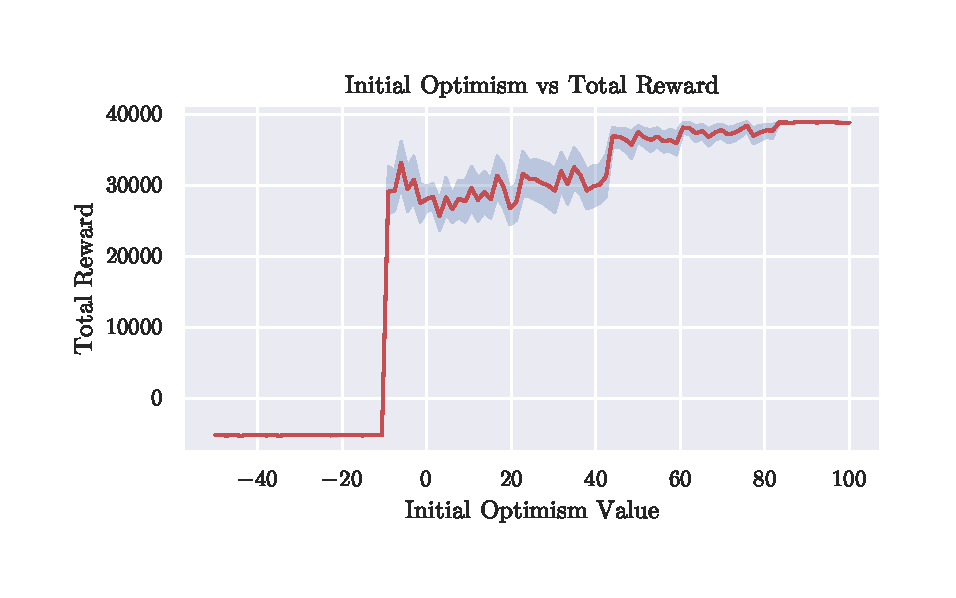
\includegraphics[trim={0 1cm 0 1cm},clip, width=\textwidth]{hyper-paramiters/inital-optimism}
  
  \caption{\label{fig:inital-optimism}}
\end{figure}


The initial optimism hyper-parameter determines the initial Q-value estimates. In essence, this is the agent's interpretation of the value of state actions before the agent has gained any experience of that state action. Since Q-learning is a bootstrapping method, depending on parameters such as the learning rate, the discount factor, and the rewards provided, initial biases may persist through more or less updates. This can be an opportunity to provide information a-priori. Value tables from previous agents can provide a head-start~\cite{deathTransfer}. While realistic initial estimates are beneficial, figure~\ref{fig:inital-optimism} shows how excessive values can be cost performance. 

When the initial estimate is larger than the expected value of each state, this is optimistic. Optimism encourages the agent to try unknown states over known states since the optimistic initial values will be strictly better than the more realistic derived value. On the other hand, pessimistic values act oppositely, discouraging exploration as known states seem better than unknown states. You can see this demonstrated in figure~\ref{fig:inital-optimism}; in the pessimistic region (left of 100), the variability is higher because the agent relies entirely on random forced exploration. 

Increasing optimism gradually decreases performance as the agent over-explores and neglects exploitation. The effect is similar for pessimism however, the performance hits a cliff after the initial estimates become negative. At this point, the agent gets stuck repeatedly choosing the same state or states. I believe this may be a consequence of several factors. Firstly, the other parameters aren't configured for this degree of pessimism, so the agent can't reach the goal based on forced exploration alone, and the pessimism stops it from exploring enough to find it. Secondly, the discount factor works in reverse when all values are negative, it encourages taking longer. Finally, Q-learning's maximisation bias may be inhibiting its ability to propagate these negative updates correctly~\cite{doubleQLearning, sutton2018reinforcement}. 


\subsection{Learning Rate \texorpdfstring{$\alpha$}{Lg}}

\begin{figure}[H]
  \centering
  
  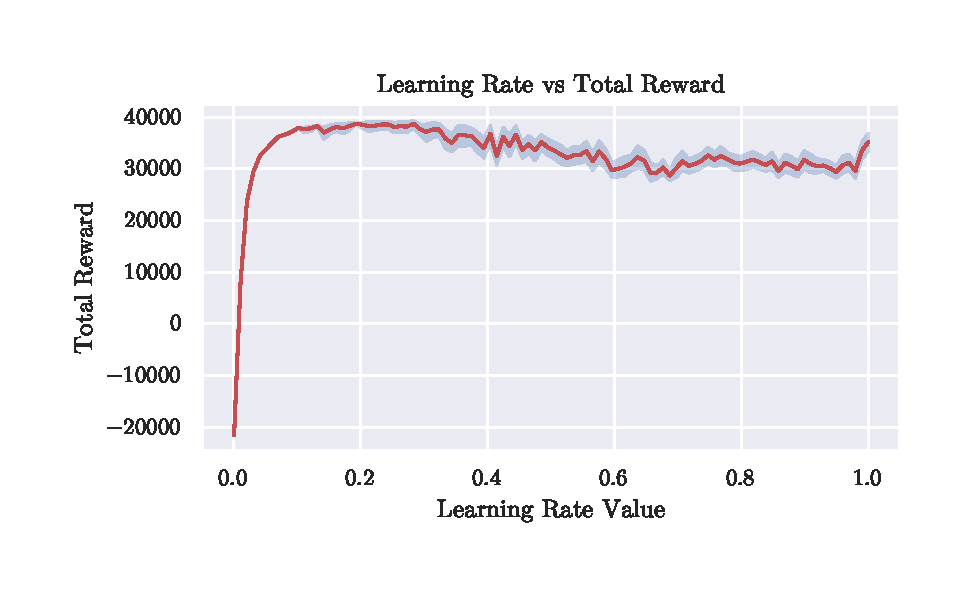
\includegraphics[trim={0 1cm 0 1cm},clip,width=\textwidth]{hyper-paramiters/learning-rate}
  
  \caption{\label{fig:learning-rate}}
\end{figure}

The learning rate $\alpha$ is another hyperparameter of Q-learning~\ref{eqn:q-learning-update-formula}. This parameter controls how much each new TD estimate will update the current estimates. For stochastic environments, getting this value right is crucial. If set too high the variability from the individual observations could lead to instability, and the Q-table may not even converge at all. The cliff dynamics that are used in this demonstration are entirely deterministic. The larger the learning rate, the fewer updates are necessary for the values to converge. However, this can be a double-edged sword because optimistic initial estimates drive most of the exploration in the current configuration. Therefore more minor updates encourage thorough but slower exploration, whereas larger updates are more rapid but lead to unstable values.

\newpage
Figure~\ref {fig:learning-rate} shows the balance of learning rate and how this impacts performance. In the range of $0.2$ to $1$, there is a plateau where the stability and speed of convergence are in balance. However, as the learning rate approaches zero the performance diminishes rapidly and the time-steps taken to learn extends. In this region, the exploration period inhibits the agent's ability to exploit the environment.

\subsection{\texorpdfstring{$\varepsilon$}{Lg}-Greedy Decay Rate}\label{edgr-section}

\begin{figure}[H]
  \centering
  
  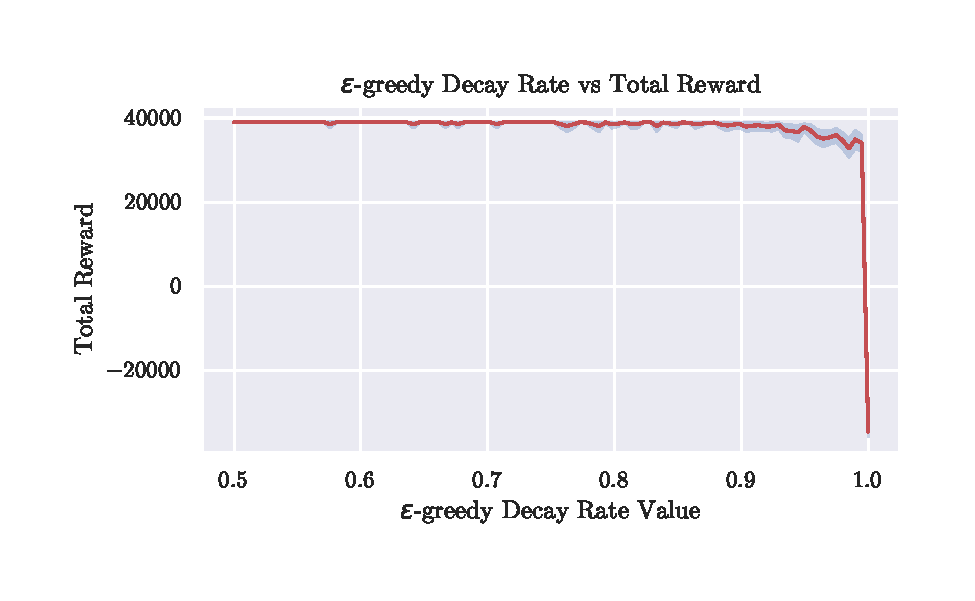
\includegraphics[trim={0 1cm 0 1cm},clip,width=\textwidth]{hyper-paramiters/epsilon-greedy-decay-full}
  
  \caption{\label{fig:epsilon-greedy-decay-full}}
\end{figure}

The $\varepsilon$-greedy decay rate (EGDR) parameter is an important and unique parameter. Figure~\ref{fig:epsilon-greedy-decay-full} demonstrates how just a minuscule amount of decay substantially improves the agent's regret and completely changes the agent's performance. Without EGDR, the cumulative reward was negative. This follows from how $\varepsilon$-greedy acts in a partially off-policy; in the cliff dynamics, the optimal policy minimises the distance travelled and, therefore travels right next to the cliff face. This path becomes problematic when $\varepsilon$-greedy introduces its off-policy exploration actions, which randomly cause the agent to select the action to jump off the cliff, incurring a significant penalty.

An on-policy method may account for the risks of selecting exploratory actions in its value estimates, encouraging the agent to give the cliff a wide berth or choose to limit the exploratory actions. However, Q-learning is an off-policy technique, so another approach is necessary. An alternative is to reduce the exploration rate once the agent has had the opportunity to learn. This application has implemented exponential decay for the exploration ratio $\varepsilon$. This exponential decay is controlled via two hyperparameters: the initial value and the decay rate. In this procedure, the exploration ratio $\varepsilon$ can be computed as: 

\begin{equation}
  \varepsilon_t = \lambda^t \cdot \varepsilon_0
\end{equation}

Where $\varepsilon_t$ is the exploration ratio at the time step $t$ and $\lambda$ represents the EGDR.

% \begin{figure}[H]
%   \centering
  
%   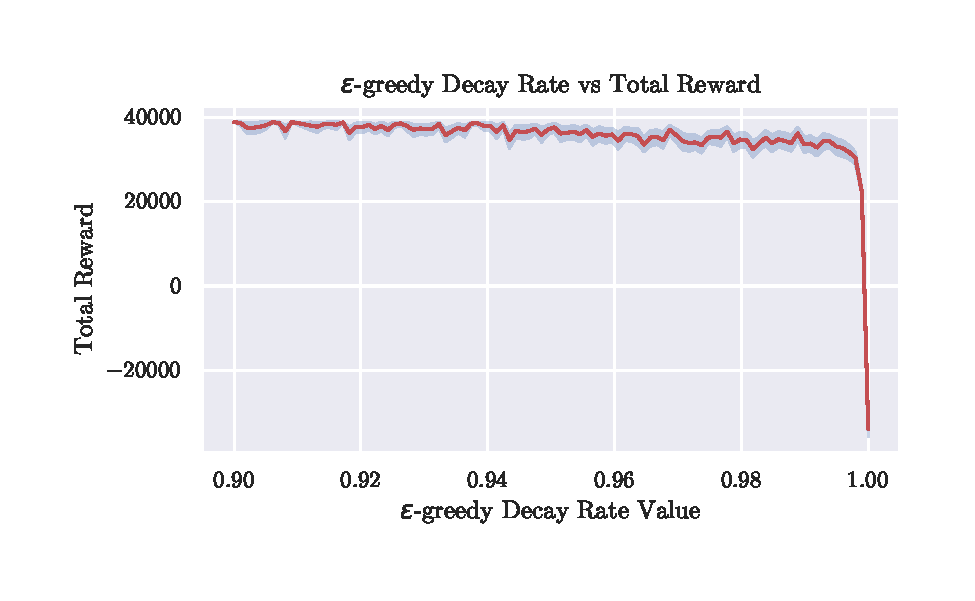
\includegraphics[trim={0 1cm 0 1cm},clip, width=\textwidth]{hyper-paramiters/epsilon-greedy-decay-top-half}
  
%   \caption{\label{fig:epsilon-greedy-decay-zoomed}Narrow range $\varepsilon$-greedy decay rate graph.}
% \end{figure}

\begin{figure}[H]
  \centering
  
  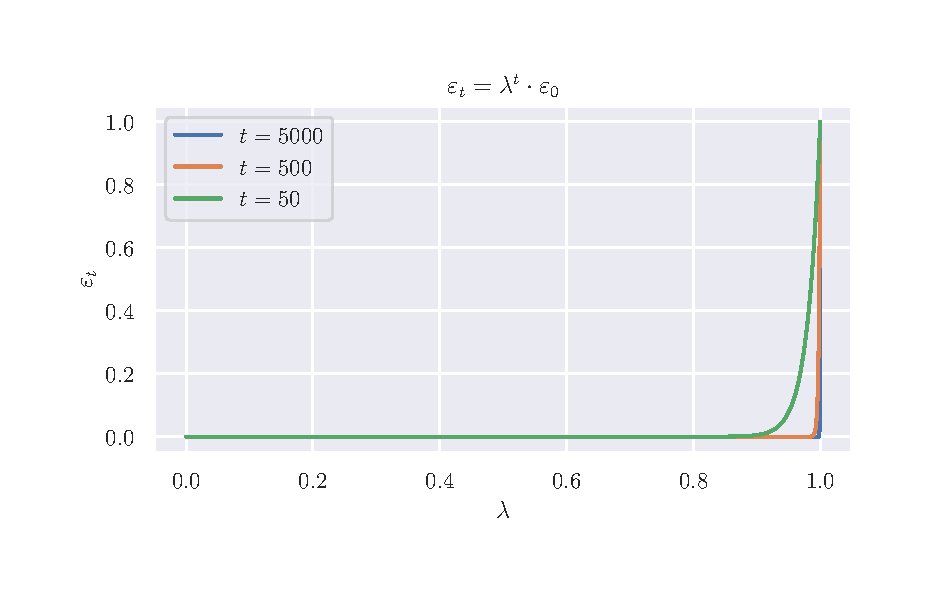
\includegraphics[trim={0 1cm 0 1cm},clip, width=\textwidth]{hyper-paramiters/example-curve.pdf}
  
  \caption{\label{fig:example-curve}}
\end{figure}


EGDR has a very striking form as there is almost no variability in performance until approximately $>0.99$ where the performance almost immediately plummets. This sharp corner follows from EGDR's compounding effects on the exploration probability. Each simulation has 5000 time steps; figure~\ref {fig:example-curve} demonstrates how with this number of time steps, all but the most extreme values will not be reduced to near zero. The figure~\ref{fig:example-curve} also shows how the EGDR parameter can control how long the agent has forced exploration. On this graph, a decay rate of $\lambda = 0.99$ would have a $60\%$ exploration probability by time step 50 whereas $\lambda < 0.6$ would have a probability if less than $1 \cdot 10^{-12}$, in other words, the figure~\ref{fig:example-curve} shows that depending on the EGDR the exploration phase may take more or less than 50 time-steps. 


I have derived this formula to predict the length of exploration:

\begin{align}
  t_{\text{exploration}} &= \log_{\lambda}(\frac{\varepsilon_{\text{min}}}{\varepsilon_0}) \\
  \varepsilon_{\text{min}} &= 1 - (1-\alpha)^{\frac{1}{d}} \label{eqn:compound-adjustment} 
\end{align}

Where $\varepsilon_{\text{min}}$ is the minimum chance of exploration to consider the agent is still exploring in each time step. This probability also compounds, so you can use the equation~\ref{eqn:compound-adjustment} to compensate for the remaining duration of the episode, where $\alpha$ is the probability of an exploratory action in the duration $d$ (number of time-steps). 



\subsection{Discount Rate \texorpdfstring{$\gamma$}{Lg}}

\begin{figure}[H]
  \centering
  
  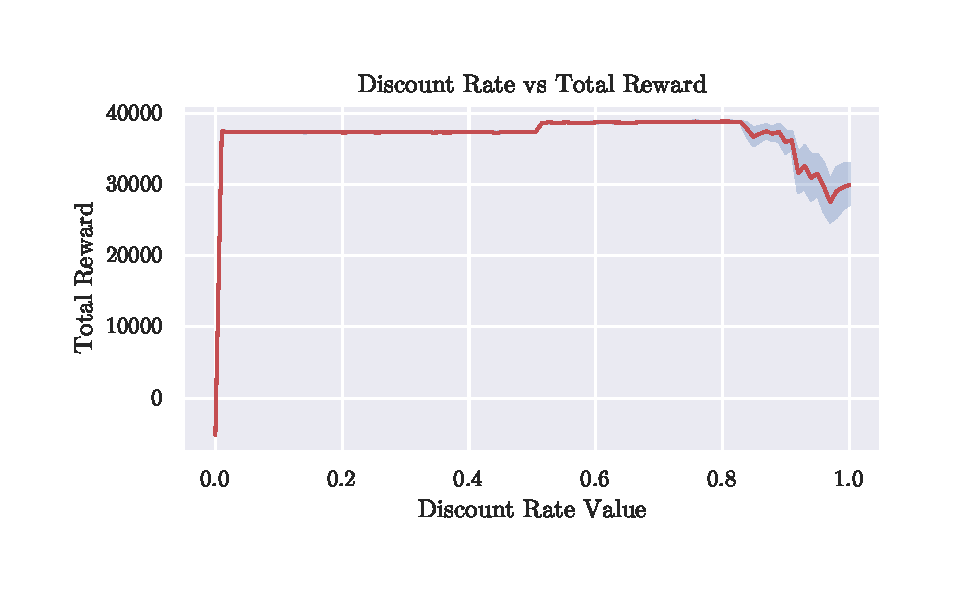
\includegraphics[trim={0 1cm 0 1cm},clip,width=\textwidth]{hyper-paramiters/discount-rate-full}
  
  \caption{\label{fig:discount-rate-full}Full range discount rate graph.}
\end{figure}

% \begin{figure}[H]
%   \centering
  
%   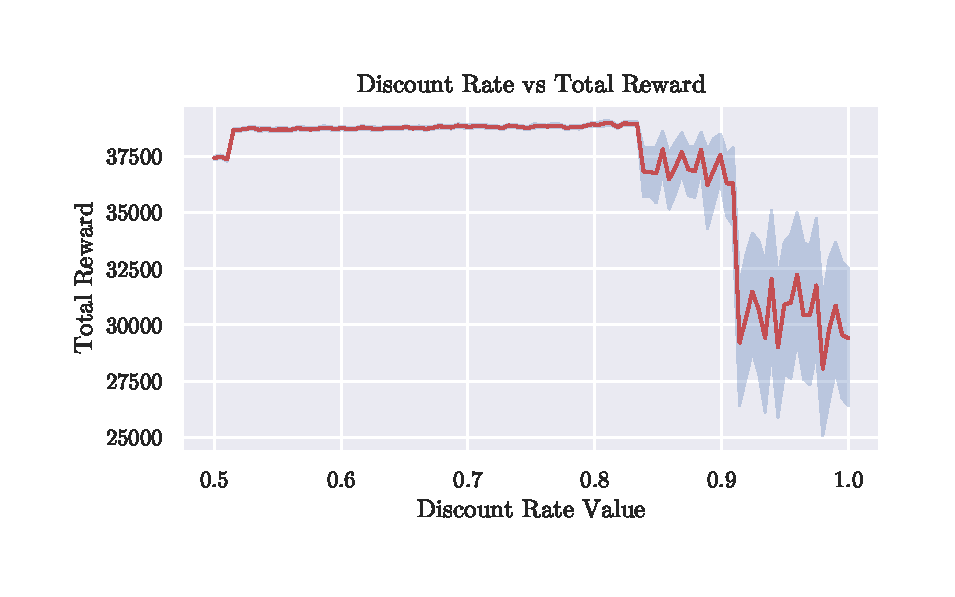
\includegraphics[trim={0 1cm 0 1cm},clip,width=\textwidth]{hyper-paramiters/discount-rate-top-half}
  
%   \caption{\label{fig:discount-rate-zoomed}Reduced range discount rate graph.}
% \end{figure}

The discount rate hyperparameter affects how much future value propagates backwards. The larger the discount rate, the more future rewards are considered, and the more far-sighted the agent becomes. Conversely the smaller the discount rate, the more short-sighted the agent's actions become~\ref{discount-rate-introduction}. When the discount rate is near zero $\gamma \approx 0$, the agent's actions have no foresight. Unfortunately, the cliff environment's reward is sparse and figure~\ref{fig:discount-rate-full} shows how having some foresight is necessary. Without it, the agent is essentially lost. 

On the other end of the spectrum, when the discount factor is large $\gamma \approx 1$, this can encourage far-sighted behaviour such as waiting. However, for the cliff environment, far-sighted behaviour was not a concern. Instead, the regret observed around $\gamma > 0.8$ in figure~\ref{fig:discount-rate-full} is explained by another factor. The bellman equations form a contraction mapping where $\gamma$ is the contraction factor~\cite{QlearningConvergance}. The result is that the discount factor is inversely proportional to the rate of convergence. Figure~\ref{discount-rate-introduction} shows how, at the extreme, the slowed convergence noticeably increases the agent's regret as the time the agent takes to learn increases.
\newpage
\section{Conclusions}

In this chapter, we have discovered that each of these three model-free exploration strategies is capable of extremely efficient exploration and exploitation. It is clear that under the right conditions, regardless of a strategy's complexity or sophistication it can perform similarly. Furthermore, each exploration strategy's performance can be incredibly sensitive to its conditions such the the environment and hyperparameters. This sensitivity can make it easy to fall into the \say{tune-and-report} trap. Instead of focusing on concrete results, reporting on general trends may be more informative. 

The parameter space has a high dimensionality and is heterogeneous, so where possible, a systematic search over the parameter space is advisable. Where this is not possible, it seems a small (relative to the rewards) amount of optimism is beneficial. A small but not negligible learning rate like $0.1$ is a good place to start. Moreover, it seems the discount rate should be roughly proportional to how sparse rewards are. 

The three strategies explored in this report vary from the simple to the state-of-the-art. On this scale, the more advanced models demonstrated better generalisation. They perform better out-of-box and have fewer tunable parameters. However, these more sophisticated models can exhibit unusual behaviour, and actions can be challenging to explain. It seems that when generalisation to varied environments is important; advanced strategies are superior. However, if the environment is fixed, a simpler strategy with tuned parameters can have similar performance and improved explainability.

\chapter{Project Analysis}
\label{chap:project-analysis}
In this project, I have created an application that implements a wide range of functionality. At its core, the application is made up of two environments and two agents. The Q-learning agent supports different exploration strategies and implements three varied strategies. Around this core, the application has many systems and functionalities that allow the user to examine and analyse the agents effectively. These systems include a fully featured graphical user interface and multiple hyperparameter tuning and report-generating systems. The GUI incorporated multiple displays, graphs and controls, and with these tools and in this project, I have been able to analyse how these agents explore. I have been able to put together this report with the background of existing research that I have explored and the analysis I have performed through this application. 

\section{Reflection of the Project Process}

With these accomplishments in sight, it can be easy to lose sight of the process. This project has spanned the last six months, and over that time, this report has incrementally developed alongside the application. The amount of progress made has varied as different factors aided or hindered the project. One of the key factors that have supported the success of this project is the application of software engineering principles in areas such as design and workflow. Importantly, these design principles have kept the application extensible to change allowing the project to be flexible and adaptable. One key example where this flexibility and adaptability has been crucial was with the user interface. As the application has grown, so has the functionality and complexity of the user interface. Unfortunately, not all of the user interface libraries could meet these growing requirements. This situation twice forced me to change the UI framework. This could have been a time-consuming procedure however, the low coupling in this application minimised the cost to switch as much of the application was unaffected. 

While the overall goals of this project are large, breaking these goals down into small but still meaningful tasks has ensured that the necessary work is completed. These smaller milestones and tasks have helped keep the project focused at the detail level. Regular meetings with my supervisor have been invaluable; they helped shape the project's direction from which the tasks are made. This organisation has helped the project progress smoothly, it has also helped steer the work in the right way as the project's direction pivoted. Originally, the project was heading towards exploring deep reinforcement learning. With some advice from Chris Watkins on the matter and the considerations mentioned in the technical decisions section~(\ref{section:technical-decsions}); I decided to redirect the project. With the help of the supervisor meetings, a new focus in exploration strategies was found as this effectively used the existing work. 
\newpage
\section{Successes and Future Enhancements}

The two environments implemented in this application have provided a good benchmark for testing an agent's ability to explore in the face of very sparse rewards and obstacles. These environments have a few commonalities; they are both a grid world and are fully deterministic. While these properties have their own merits and use-cases this project would be enhanced with a broader and more diverse collection of environments. Importantly, stochastic environments would test the exploration of these agents in a new way, and the effects of learning rates would change. There are many famous reinforcement learning environments; some are stochastic, such as river-swim, and many are not based in a grid world, like the cart pole balancing problem. Many RL environments such as these traditional ones, Atari games and many more are collated into a Python library called gymnasium~\cite{gym}. If the application integrates the gymnasium library with its dynamics system, this would provide a substantial improvement. Firstly, the application would allow access to a wide range of environments. Secondly, these same environments are widely used in RL research, helping to standardise this work and allow for more direct comparisons. However, the gymnasium library would not just plug into the existing code. The interface is substantially different enough from the application that some structural changes must be made. While an adapter could shim the differences, a tight integration would really enrich this project. In summation, integrating the gymnasium library would provide the project a leap forward in terms of the number of environments and their variety; however, doing this right involves attention and has unfortunately fallen outside of this project's scope. 

Provided with enough time and resources, implementing deep reinforcement learning could provide this project with a new dimension of research and greater depth. An excellent place to start would be DBMF-BPI. This algorithm is a deep reinforcement learning extension to the MF-BPI strategy~\cite{modelFree}. DBMF-BPI has already been implemented in Python, and its relation to the MF-BPI strategy makes it a great candidate for incorporation into this application. This project would also benefit from a wider variety of reinforcement learning algorithms, such as Monti-carlo, Actor-Critic or even model-based algorithms. However, implementing and analysing these algorithms would substantially increase this project's scope, and they were unobtainable under the current time and resource constraints. That said, these extensions would benefit from the prior work done on this project. The foundations laid for the other algorithms would likely need only slight adaptations to support this new work. 
\section{Conclusion}

This project has explored reinforcement learning, some of the broader machine learning field as well as topics such as psychology and professional issues. However, the project has focused on the exploration of learning agents in a Markov Decision Process. To this end, the project has looked at Q-learning with different exploration strategies and analysed the challenges of efficient exploration. With this in mind, the project has met its objectives. Through this project, I have learned and gained a lot. I believe this project has been successful and has the potential for further success with extensions. 

%%%% ADD YOUR BIBLIOGRAPHY HERE
\newpage

\bibliographystyle{IEEEtran}
\bibliography{refrences}
\addcontentsline{toc}{chapter}{Bibliography}

\appendix


\chapter{User Manual}

\hypertarget{running-the-program}{%
\subsection{Running the Program}\label{running-the-program}}

\begin{quote}
Note: This guide is for those only interested in using the application,
see \protect\hyperlink{development}{Development} for a development
workflow.
\end{quote}

This project requires Python 3.10. Python installers can be found
\href{https://www.python.org/downloads/}{here}. The program has a GU

\begin{quote}
If you encounter issues or don't want to install this program locally
there is a docker file \href{../.devcontainer/Dockerfile}{here}. This
docker file specifies the environment and all the tooling for this
project.
\end{quote}

You can install and run the project with a Python package manager such
as \texttt{pipx} or \texttt{poetry}. we will be using \texttt{pipx} here
because of its simplicity. There is a guide
\href{https://pypa.github.io/pipx/installation/}{here} on how you can
install \texttt{pipx}.

once \texttt{pipx} is installed open your terminal and navigate to this
folder (\texttt{code}) and run this command to start the program

\begin{Shaded}
\begin{Highlighting}[]
\ExtensionTok{python3}\NormalTok{ {-}m pipx run {-}{-}spec . start}
\end{Highlighting}
\end{Shaded}

\hypertarget{project-structure}{%
\subsection{Project Structure}\label{project-structure}}

the project is mostly hierarchical with related features being located
in the same or nearby folders (packages). the root folder \texttt{code}
contains all the meta configuration for this project, this includes -
\texttt{pyproject.toml}: which specifies what dependencies the program
needs. the entry points and other tooling configurations. -
\texttt{setup.cfg}: contains the configuration for tools that have not
migrated to the PEP 518 (\texttt{pyproject.toml}) standard yet -
\texttt{.pre-commit-config}: specifies what should be run before a
commit is allowed. - \texttt{.gitignore}: excludes certain files from
being added to the git repository.

the \texttt{code} folder contains two more important folders
\texttt{src} and \texttt{tests}. tests contains all the tests and the
related mocks necessary, code in the tests package is not used at
runtime.

\texttt{src} folder contains everything necessary at runtime, these are
in four main parts: - \texttt{model}: where all of the state and
learning functionality is stored - \texttt{view}: where all of the GUI
code for visualizing the reinforcement learning is stored -
\texttt{controller}: the code that updates the model with the user's
input, this is the code that unites the model and view. -
\texttt{entry\ points}: this is where execution starts. There are two,
the main entry point and one for profiling the code.

\texttt{src} is mostly code however it also includes the application's
config \href{./src/config.toml}{\texttt{src/config.toml}} and the icon
files used by the program. This
\href{./src/config.toml}{\texttt{src/config.toml}} is where important
configuration options for the application are determined such as the
size of the grid world. The icons are from Flaticon and require the
following attribution:

UIcons by \href{https://www.flaticon.com/uicons}{Flaticon}

\newpage
\hypertarget{documentation}{%
\subsection{Documentation}\label{documentation}}

Documentation is written alongside the code with doc-strings, in the
Google docstring format. This can be built into a complete documentation
site. a package called \texttt{mkdocs} has been configured for building
this site.

The last build of the docs is at \texttt{code/docs} you can open these
files directly or run one of the following commands to start a local
server then open \url{http://localhost:3000} in your browser to view the
documentation.

To start a local server of the last build you can run.

\begin{Shaded}
\begin{Highlighting}[]
\ExtensionTok{python3}\NormalTok{ {-}m http.server {-}{-}directory docs 3000}
\end{Highlighting}
\end{Shaded}

Alternatively use the following command to get the latest docs as a
local server.

\begin{Shaded}
\begin{Highlighting}[]
\ExtensionTok{poetry}\NormalTok{ run mkdocs serve {-}a localhost:3000}
\end{Highlighting}
\end{Shaded}

\hypertarget{development}{%
\subsection{Development}\label{development}}

To develop on this project I recommend using
\href{https://code.visualstudio.com/download}{Visual Studio Code} and
the provided
\href{https://code.visualstudio.com/docs/devcontainers/containers}{development
container}. using VS Code and this development container standardises
the environment and avoids device-specific issues and this repository is
configured for a VS Code workflow.

If not using VS Code, the required tools are: - Python 3.10, including:
- Virtual environments (\texttt{venv}) - \texttt{tkinter}/ Tcl -
\texttt{pip} - \texttt{poetry} - \texttt{pre-commit}

\hypertarget{poetry}{%
\subsubsection{Poetry}\label{poetry}}

Poetry is a Python package manager and it manages the Python retirements
of this project.

When you first start you will need to run the following command to
install the dependencies

\begin{Shaded}
\begin{Highlighting}[]
\ExtensionTok{poetry}\NormalTok{ install}
\end{Highlighting}
\end{Shaded}

you will also need to run the following command, to ensure each commit
meets the linting requirements:

\begin{Shaded}
\begin{Highlighting}[]
\ExtensionTok{poetry}\NormalTok{ run pre{-}commit install}
\end{Highlighting}
\end{Shaded}

To run the project run:

\begin{Shaded}
\begin{Highlighting}[]
\ExtensionTok{poetry}\NormalTok{ run start}
\end{Highlighting}
\end{Shaded}

\hypertarget{code-quality-tooling}{%
\subsubsection{Code quality tooling}\label{code-quality-tooling}}

To avoid bugs and enforce consistency this project has a number of
tools. these tools are configured with \texttt{pre-commit} to run
together before each commit, all tools must pass before a commit can be
pushed.

the tools are:

\begin{longtable}[]{@{}lll@{}}
\toprule
Tool & Description & command\tabularnewline
\midrule
\endhead
\texttt{black} & Formats the code in a consistent way. &
\texttt{poetry\ run\ black\ src}\tabularnewline
\texttt{pytest} & Ensures all tests are passing. &
\texttt{poetry\ run\ pytest\ -\/-cov}\tabularnewline
\texttt{flake8} & Lints the code, ensure that it meets standard. &
\texttt{poetry\ run\ flake8}\tabularnewline
\texttt{mypy} & Ensures all static types are correct. &
\texttt{poetry\ run\ mypy}\tabularnewline
\bottomrule
\end{longtable}

they can be all run together with:

\begin{Shaded}
\begin{Highlighting}[]
\ExtensionTok{pre{-}commit}\NormalTok{ run {-}{-}all{-}files}
\end{Highlighting}
\end{Shaded}

\hypertarget{tips}{%
\subsubsection{Tips}\label{tips}}

\href{https://readthedocs.org/projects/wemake-python-styleguide/}{we
make python} is the style guide that this project follows have a look at
the
\href{https://wemake-python-styleguide.readthedocs.io/en/latest/}{docs
here} for an explanation of their rules, some I have found to be
contradictory with other tooling or excessively restrictive so I have
disabled them

if the code needs formatting then in the first pass of pre-commit it
will update the code but it will fail the test because it needed to be
updated, re-run pre-commit/ try committing again and it will often
succeed


\chapter{Diary}





\hypertarget{week-01-180923}{%
  \subsubsection{Week 01 (18/09/23)}\label{week-01-180923}}

\begin{itemize}
  \tightlist
  \item
        (Tue 19) Attended first lecture
  \item
        (Thu 21) Started reading Reinforcement Learning in 'Machine Learning'
        by Tom Mitchell
  \item
        (Fri 22) Finished reading Reinforcement Learning in 'Machine Learning'
        by Tom Mitchell
\end{itemize}

\hypertarget{week-02-250923}{%
  \subsubsection{Week 02 (25/09/23)}\label{week-02-250923}}

\begin{itemize}
  \tightlist
  \item
        (Mon 25) Decided on project idea

        \begin{itemize}
          \tightlist
          \item
                Started draft project plan
          \item
                Abstract
          \item
                Risks
        \end{itemize}
  \item
        (Tue 26) First meeting with Anand

        \begin{itemize}
          \tightlist
          \item
                Started putting together timeline
          \item
                Started reading Reinforcement Learning An Introduction by Richard S.
                Sutton and Andrew G. Barto
        \end{itemize}
  \item
        (Wed 27)

        \begin{itemize}
          \tightlist
          \item
                Attended second lecture
          \item
                moved project plan over to LaTeX
        \end{itemize}
  \item
        (Thu 28) Worked on project plan report

        \begin{itemize}
          \tightlist
          \item
                improved bibliography
        \end{itemize}
\end{itemize}

\hypertarget{week-03-021023}{%
  \subsubsection{Week 03 (02/10/23)}\label{week-03-021023}}

\begin{itemize}
  \tightlist
  \item
        (Tue 03) worked on project plan

        \begin{itemize}
          \tightlist
          \item
                Put together risks section
          \item
                put together timeline
        \end{itemize}
  \item
        (Wed 04) submitted project plan to Anand
  \item
        (Thu 05) Finished project plan

        \begin{itemize}
          \tightlist
          \item
                Improved abstract
          \item
                improved bibliography
        \end{itemize}
\end{itemize}

\hypertarget{week-04-091023}{%
  \subsubsection{Week 04 (09/10/23)}\label{week-04-091023}}

\begin{itemize}
  \tightlist
  \item
        (Wed 11) Gitlab

        \begin{itemize}
          \tightlist
          \item
                Attended lecture about gitlab
          \item
                Moved Code to GitLab

                \begin{itemize}
                  \tightlist
                  \item
                        setup credentials
                  \item
                        updated remotes
                  \item
                        pushed code
                \end{itemize}
        \end{itemize}
  \item
        (Thu 12) Created Initial Interim report from template

        \begin{itemize}
          \tightlist
          \item
                Finished chapter one from Sutton Barto book
        \end{itemize}
\end{itemize}

\hypertarget{week-05-161023}{%
  \subsubsection{Week 05 (16/10/23)}\label{week-05-161023}}

\begin{itemize}
  \tightlist
  \item
        (Mon 16) Continued reading Sutton Barto book

        \begin{itemize}
          \tightlist
          \item
                chapter 2 and some of chapter 3
        \end{itemize}
  \item
        (Wed 18) Continued reading

        \begin{itemize}
          \tightlist
          \item
                finished Chapter 3
          \item
                attended lecture about testing
        \end{itemize}
  \item
        (Thu 19)

        \begin{itemize}
          \tightlist
          \item
                Second Meeting with Anand
        \end{itemize}
  \item
        (Fri 20) Continued reading read subsections on policy improvement
\end{itemize}

\hypertarget{week-06-231023}{%
  \subsubsection{Week 06 (23/10/23)}\label{week-06-231023}}

\begin{itemize}
  \tightlist
  \item
        (Mon 23)

        \begin{itemize}
          \tightlist
          \item
                Continued reading Sutton Barto book

                \begin{itemize}
                  \tightlist
                  \item
                        read chapters 4,6 and skimmed 5
                \end{itemize}
          \item
                Met Anand to discuss my project plan
        \end{itemize}
\end{itemize}

\hypertarget{week-07-301023}{%
  \subsubsection{Week 07 (30/10/23)}\label{week-07-301023}}

\begin{itemize}
  \tightlist
  \item
        (Thu 02)

        \begin{itemize}
          \tightlist
          \item
                Started MDP Report
          \item
                Third Meeting with Anand
        \end{itemize}
  \item
        (Weekend 4-5)

        \begin{itemize}
          \tightlist
          \item
                Completed MDP Report
        \end{itemize}
\end{itemize}

\hypertarget{week-08-061023}{%
  \subsubsection{Week 08 (06/10/23)}\label{week-08-061023}}

\begin{itemize}
  \tightlist
  \item
        (Mon 06) Started report on the policy and value functions
  \item
        (Tue 07) Completed policy and value report
  \item
        (Wed 08)

        \begin{itemize}
          \tightlist
          \item
                Completed policy and value report
          \item
                Started Q-learning report
        \end{itemize}
  \item
        (Thu 09)

        \begin{itemize}
          \tightlist
          \item
                Completed Q-learning report
          \item
                Started code setup
        \end{itemize}
  \item
        (Weekend 10-11) continued setting up code
\end{itemize}

\hypertarget{week-09-131123}{%
  \subsubsection{Week 09 (13/11/23)}\label{week-09-131123}}

\begin{itemize}
  \tightlist
  \item
        (Mon 13)

        \begin{itemize}
          \tightlist
          \item
                Completed code setup
        \end{itemize}
  \item
        (Tue 14)

        \begin{itemize}
          \tightlist
          \item
                Started vertical slice
        \end{itemize}
  \item
        (Wed 15)

        \begin{itemize}
          \tightlist
          \item
                Started writing collection dynamics method
        \end{itemize}
  \item
        (Thu 16)

        \begin{itemize}
          \tightlist
          \item
                Completed collection dynamics
          \item
                Started implementing value iteration
          \item
                Fourth meeting with Anand
        \end{itemize}
  \item
        (Fri 17)

        \begin{itemize}
          \tightlist
          \item
                completed value iteration agent
        \end{itemize}
\end{itemize}

\hypertarget{week-10-201123}{%
  \subsubsection{Week 10 (20/11/23)}\label{week-10-201123}}

\begin{itemize}
  \tightlist
  \item
        (Mon 20)

        \begin{itemize}
          \tightlist
          \item
                Created controllers to tie view and model together.
          \item
                Tried to display grid with canvas approach

                \begin{itemize}
                  \tightlist
                  \item
                        ran into rendering limitations, with many rectangles rectangles
                        kivy started to have issues with rendering the icons.
                \end{itemize}
        \end{itemize}
  \item
        (Tue 21) tried widget based approach

        \begin{itemize}
          \tightlist
          \item
                Tried using kivy's layout widgets to display the grid
          \item
                while the icons were no longer an issue positioning the grid became
                impossible
          \item
                investigated kivy alternatives
        \end{itemize}
  \item
        (Wed 22) Pivoted to using tkinter

        \begin{itemize}
          \tightlist
          \item
                remade exiting UI in tkinter and updated tooling for working with
                tkinter
          \item
                completed grid world display widget
        \end{itemize}
  \item
        (Thu 23)

        \begin{itemize}
          \tightlist
          \item
                Added button that progresses the state over time.
          \item
                Created methods to provide the Q-value information to the view,
                allowing for visualisation.
        \end{itemize}
  \item
        (Fri 24)

        \begin{itemize}
          \tightlist
          \item
                Started adding Q-value visualisation code,
          \item
                Optimised value iteration code with numba
          \item
                Reworked how cells are provided their information
        \end{itemize}
\end{itemize}

\hypertarget{week-11-271123}{%
  \subsubsection{Week 11 (27/11/23)}\label{week-11-271123}}

\begin{itemize}
  \tightlist
  \item
        (Mon 27) Created tooltip to provide state value information and fixed
        origin inconsistency from the move to tkinter.
  \item
        (Tue 28) Completed system for allowing the user to select between
        different types of displays
  \item
        (Wed 29)

        \begin{itemize}
          \tightlist
          \item
                Improved code \texttt{README} and improved usability
          \item
                Implemented the Q-learning agent with
          \item
                Added simultaneous agents to speed up learning
          \item
                Added opening to project report
        \end{itemize}
  \item
        (Thu 30)

        \begin{itemize}
          \tightlist
          \item
                Improved Interim Report
          \item
                Fifth meeting with Anand

                \begin{itemize}
                  \tightlist
                  \item
                        Anand noticed how the simultaneous agents deviated for the
                        literature
                \end{itemize}
        \end{itemize}
  \item
        (Fri 01) Refactor

        \begin{itemize}
          \tightlist
          \item
                Removed the simultaneous agents feature
          \item
                focused on Improving performance in other ways:

                \begin{itemize}
                  \tightlist
                  \item
                        Split MVC across different processes to avoid the GIL
                  \item
                        Improved rendering approach with Pillow no more odd layout and
                        widgets
                \end{itemize}
          \item
                Started making presentation
        \end{itemize}
  \item
        (Sat 02)

        \begin{itemize}
          \tightlist
          \item
                Completed presentation slides
          \item
                Practised presentation
        \end{itemize}
\end{itemize}

\hypertarget{week-12-081223}{%
  \subsection{Week 12 (08/12/23)}\label{week-12-081223}}

\begin{itemize}
  \tightlist
  \item
        (Mon 04)

        \begin{itemize}
          \tightlist
          \item
                Practised presentation
          \item
                Gave presentation
        \end{itemize}
  \item
        (Fri 08)

        \begin{itemize}
          \tightlist
          \item
                Prepared work for Interim submission
        \end{itemize}
\end{itemize}




\label{endpage}



\end{document}

\end{article}
